\documentclass[10pt,a4paper]{article}

\usepackage[T1]{fontenc}
\usepackage[utf8]{inputenc}
\usepackage{lmodern}
\usepackage[margin=2.3cm]{geometry}
\usepackage{amsmath,amssymb}
\usepackage{graphicx}
\usepackage{booktabs}
\usepackage{array}
\usepackage{url}
\usepackage{xcolor}
\usepackage{microtype}
\usepackage[hidelinks]{hyperref}
\usepackage{orcidlink}
\usepackage{caption}
\usepackage{algorithm}
\usepackage{algpseudocode}
\usepackage{amsthm}
\newtheorem{proposition}{Proposition}
\newtheorem{conjecture}{Conjecture}
\captionsetup{font=small,labelfont=bf}
\setlength{\parskip}{0.4em}
\setlength{\parindent}{0pt}
\setlength{\emergencystretch}{2em}

\graphicspath{{../figures/}}
% Generated by data/measure.py from warm.json. Do not edit.
\newcommand{\nGeo}{66}
\newcommand{\nGen}{60}
\newcommand{\nBench}{6}
\newcommand{\nSeeds}{3}
\newcommand{\budget}{60}
\newcommand{\trapsMin}{49}
\newcommand{\trapsMax}{1024}
\newcommand{\trapsMed}{275}
\newcommand{\benchTrapsMax}{1024}
\newcommand{\benchTrapsMin}{36}
\newcommand{\itRTwelve}{14}
\newcommand{\itRTwelveLo}{14}
\newcommand{\itRTwelveHi}{14}
\newcommand{\itRTwelveQa}{13}
\newcommand{\itRTwelveQb}{15}
\newcommand{\neverRTwelve}{6.1}
\newcommand{\neverGeoRTwelve}{4}
\newcommand{\finRTwelve}{0.00013}
\newcommand{\effmRTwelve}{0.790}
\newcommand{\itRThree}{7.5}
\newcommand{\itRThreeLo}{6}
\newcommand{\itRThreeHi}{10.5}
\newcommand{\itRThreeQa}{5}
\newcommand{\itRThreeQb}{61}
\newcommand{\neverRThree}{32.8}
\newcommand{\neverGeoRThree}{21}
\newcommand{\finRThree}{0.217}
\newcommand{\effmRThree}{0.757}
\newcommand{\itNThree}{8}
\newcommand{\itNThreeLo}{7}
\newcommand{\itNThreeHi}{17}
\newcommand{\itNThreeQa}{5}
\newcommand{\itNThreeQb}{61}
\newcommand{\neverNThree}{34.8}
\newcommand{\neverGeoNThree}{23}
\newcommand{\finNThree}{0.216}
\newcommand{\effmNThree}{0.756}
\newcommand{\itNTwelve}{14}
\newcommand{\itNTwelveLo}{14}
\newcommand{\itNTwelveHi}{14.5}
\newcommand{\itNTwelveQa}{13}
\newcommand{\itNTwelveQb}{15}
\newcommand{\neverNTwelve}{4.5}
\newcommand{\neverGeoNTwelve}{3}
\newcommand{\finNTwelve}{0.000222}
\newcommand{\effmNTwelve}{0.791}
\newcommand{\ratioRoverN}{1.75}
\newcommand{\ratioRoverNLo}{0.85}
\newcommand{\ratioRoverNHi}{2}
\newcommand{\ratioRoverRThree}{1.87}
\newcommand{\ratioRoverRThreeLo}{1.38}
\newcommand{\ratioRoverRThreeHi}{2.33}
\newcommand{\ratioRThreeoverN}{0.94}
\newcommand{\ratioRThreeoverNLo}{0.56}
\newcommand{\ratioRThreeoverNHi}{1.07}
\newcommand{\ratioRoverNTwelve}{1}
\newcommand{\ratioRoverNTwelveLo}{1}
\newcommand{\ratioRoverNTwelveHi}{1}
\newcommand{\signARN}{37}
\newcommand{\signBRN}{23}
\newcommand{\signTRN}{6}
\newcommand{\signPRN}{0.092}
\newcommand{\signARThreeN}{6}
\newcommand{\signBRThreeN}{13}
\newcommand{\signTRThreeN}{47}
\newcommand{\signPRThreeN}{0.17}
\newcommand{\signARRThree}{40}
\newcommand{\signBRRThree}{17}
\newcommand{\signTRRThree}{9}
\newcommand{\signPRRThree}{0.0032}
\newcommand{\signARNTwelve}{8}
\newcommand{\signBRNTwelve}{14}
\newcommand{\signTRNTwelve}{44}
\newcommand{\signPRNTwelve}{0.29}
\newcommand{\effdRThree}{4.2}
\newcommand{\effdNThree}{4.3}
\newcommand{\effdNTwelve}{0.1}
\newcommand{\effdNThreeRThree}{0.1}
\newcommand{\recRatio}{1.75}
\newcommand{\recEff}{4.2}
\newcommand{\recUni}{0.7}
\newcommand{\onnxBytes}{338\,987}
\newcommand{\parityMax}{9.8\times10^{-4}}
\newcommand{\nParams}{80\,899}
\newcommand{\trainSteps}{6000}
\newcommand{\runtimeMin}{37.6}
\newcommand{\nWorkers}{12}
\newcommand{\genItRTwelve}{14}
\newcommand{\genItNThree}{8.5}
\newcommand{\genItRThree}{8}
\newcommand{\benchItRTwelve}{13.5}
\newcommand{\benchItNThree}{5}
\newcommand{\benchItRThree}{6}
\newcommand{\swOne}{61}
\newcommand{\swOneNever}{76.7}
\newcommand{\swOneFin}{34.3}
\newcommand{\swTwo}{61}
\newcommand{\swTwoNever}{61.1}
\newcommand{\swTwoFin}{2.32}
\newcommand{\swThree}{9.5}
\newcommand{\swThreeNever}{41.1}
\newcommand{\swThreeFin}{0.512}
\newcommand{\swFour}{8}
\newcommand{\swFourNever}{28.9}
\newcommand{\swFourFin}{0.202}
\newcommand{\swSix}{10}
\newcommand{\swSixNever}{14.4}
\newcommand{\swSixFin}{0.0742}
\newcommand{\swEight}{11}
\newcommand{\swEightNever}{12.2}
\newcommand{\swEightFin}{0.00997}
\newcommand{\swTwelve}{14}
\newcommand{\swTwelveNever}{7.8}
\newcommand{\swTwelveFin}{0.00013}
\newcommand{\swnOne}{61}
\newcommand{\swnOneNever}{80}
\newcommand{\swnOneFin}{52.2}
\newcommand{\swnTwo}{61}
\newcommand{\swnTwoNever}{70}
\newcommand{\swnTwoFin}{20.1}
\newcommand{\swnThree}{10.5}
\newcommand{\swnThreeNever}{40}
\newcommand{\swnThreeFin}{0.213}
\newcommand{\swnFour}{9}
\newcommand{\swnFourNever}{23.3}
\newcommand{\swnFourFin}{0.18}
\newcommand{\swnSix}{10}
\newcommand{\swnSixNever}{20}
\newcommand{\swnSixFin}{0.0371}
\newcommand{\swnEight}{12}
\newcommand{\swnEightNever}{16.7}
\newcommand{\swnEightFin}{0.0352}
\newcommand{\swnTwelve}{14}
\newcommand{\swnTwelveNever}{6.7}
\newcommand{\swnTwelveFin}{1.91e-05}
\newcommand{\OOneMed}{5.5}
\newcommand{\OOneMin}{2}
\newcommand{\OOneMax}{61}
\newcommand{\OThreeMed}{5.5}
\newcommand{\OThreeMin}{2}
\newcommand{\OThreeMax}{61}
\newcommand{\OTwelveMed}{13}
\newcommand{\OTwelveMin}{2}
\newcommand{\OTwelveMax}{61}
\newcommand{\ORMed}{14}
\newcommand{\ORMin}{5}
\newcommand{\ORMax}{61}
\newcommand{\ORThreeMed}{11.5}
\newcommand{\ORThreeMin}{4}
\newcommand{\ORThreeMax}{61}
\newcommand{\ONetMed}{7}
\newcommand{\ONetMin}{4}
\newcommand{\ONetMax}{61}
\newcommand{\wTwelveHold}{10}
\newcommand{\wTwelveN}{10}
\newcommand{\wTwelveSMed}{0.71}
\newcommand{\wTwelveKMed}{2}
\newcommand{\wTwelveKMin}{2}
\newcommand{\wTwelveKMax}{21}
\newcommand{\wTwelveItMed}{14}
\newcommand{\wThreeHold}{10}
\newcommand{\wThreeN}{10}
\newcommand{\wThreeSMed}{1.43}
\newcommand{\wThreeKMed}{3}
\newcommand{\wThreeKMin}{3}
\newcommand{\wThreeKMax}{16}
\newcommand{\wThreeItMed}{11.5}
\newcommand{\woTwelveHold}{10}
\newcommand{\woTwelveN}{10}
\newcommand{\woTwelveSMed}{0.67}
\newcommand{\woTwelveKMed}{4}
\newcommand{\woTwelveKMin}{3}
\newcommand{\woTwelveKMax}{52}
\newcommand{\woTwelveItMed}{13}
\newcommand{\woThreeHold}{10}
\newcommand{\woThreeN}{10}
\newcommand{\woThreeSMed}{0.8}
\newcommand{\woThreeKMed}{5.5}
\newcommand{\woThreeKMin}{3}
\newcommand{\woThreeKMax}{57}
\newcommand{\woThreeItMed}{5.5}
\newcommand{\nPixGen}{256}
\newcommand{\padGen}{2}
\newcommand{\lambdaNm}{850}
\newcommand{\focalMm}{250}
\newcommand{\pitchUm}{12.5}
\newcommand{\chirpFinal}{79.96}
\newcommand{\trRTwelveOne}{30.35}
\newcommand{\trRTwelveTwo}{15.61}
\newcommand{\trRTwelveThree}{9.85}
\newcommand{\trRTwelveFour}{8.4}
\newcommand{\trRTwelveFive}{6.92}
\newcommand{\trRTwelveSix}{5.92}
\newcommand{\trRTwelveEleven}{2.85}
\newcommand{\trRTwelveTwelve}{2.61}
\newcommand{\trRTwelveThirteen}{1.2}
\newcommand{\trRTwelveFourteen}{0.67}
\newcommand{\trRThreeOne}{30.35}
\newcommand{\trRThreeTwo}{15.61}
\newcommand{\trRThreeThree}{9.85}
\newcommand{\trRThreeFour}{3.92}
\newcommand{\trRThreeFive}{2.17}
\newcommand{\trRThreeSix}{1.37}
\newcommand{\trRThreeEleven}{0.46}
\newcommand{\trRThreeTwelve}{0.45}
\newcommand{\trRThreeThirteen}{0.42}
\newcommand{\trRThreeFourteen}{0.42}
\newcommand{\trNThreeOne}{31.11}
\newcommand{\trNThreeTwo}{16.5}
\newcommand{\trNThreeThree}{10.09}
\newcommand{\trNThreeFour}{4.25}
\newcommand{\trNThreeFive}{2.51}
\newcommand{\trNThreeSix}{1.69}
\newcommand{\trNThreeEleven}{0.51}
\newcommand{\trNThreeTwelve}{0.46}
\newcommand{\trNThreeThirteen}{0.42}
\newcommand{\trNThreeFourteen}{0.42}
\newcommand{\trNTwelveOne}{31.11}
\newcommand{\trNTwelveTwo}{16.5}
\newcommand{\trNTwelveThree}{10.09}
\newcommand{\trNTwelveFour}{8.8}
\newcommand{\trNTwelveFive}{7.4}
\newcommand{\trNTwelveSix}{6.28}
\newcommand{\trNTwelveEleven}{3.09}
\newcommand{\trNTwelveTwelve}{2.79}
\newcommand{\trNTwelveThirteen}{1.37}
\newcommand{\trNTwelveFourteen}{0.84}
\newcommand{\swThreeEx}{6.5}
\newcommand{\swFourEx}{4}
\newcommand{\swSixEx}{4}
\newcommand{\swEightEx}{3}
\newcommand{\swTwelveEx}{2}
\newcommand{\capRNotN}{1}
\newcommand{\capNNotR}{3}
\newcommand{\capBoth}{20}
\newcommand{\OTwelveGain}{1}
\newcommand{\itMFour}{61}
\newcommand{\itMFourLo}{61}
\newcommand{\itMFourHi}{61}
\newcommand{\neverMFour}{100}
\newcommand{\finMFour}{16.3}
\newcommand{\effmMFour}{0.821}
\newcommand{\itMSix}{30}
\newcommand{\itMSixLo}{27}
\newcommand{\itMSixHi}{36}
\newcommand{\neverMSix}{6.6}
\newcommand{\finMSix}{0.472}
\newcommand{\effmMSix}{0.808}
\newcommand{\trainMinutes}{30.8}
\newcommand{\trainFirstLoss}{2.54}
\newcommand{\trainLastLoss}{0.97}
\newcommand{\trainSigNet}{0.176}
\newcommand{\trainSigRand}{0.143}
\newcommand{\trainSigNetFirst}{9.2}
\newcommand{\trainSigRandFirst}{12}
\newcommand{\ctrlRTwelve}{14}
\newcommand{\ctrlRThree}{9}
\newcommand{\ctrlNThree}{16.5}
\newcommand{\recMedModel}{8}
\newcommand{\recMedRandom}{14}


% Page-1 header block (conventions/manuscript-header-standard.md). The four document macros are set by the
% publishing tool when the version DOI is reserved.
\newcommand{\doctype}{Preprint}
\newcommand{\docversion}{v0.01}
\newcommand{\docdate}{3 November 2026}
\newcommand{\versiondoi}{10.5281/zenodo.pending}
\newcommand{\conceptdoi}{10.5281/zenodo.pending}
\newcommand{\docrepo}{github.com/fsantibanezleal/CEFOP\_DinHot}
\newcommand{\headerblock}{%
\begin{center}
\fbox{\parbox{0.94\textwidth}{\small\raggedright
\textbf{\doctype} \quad$\cdot$\quad \docversion, \docdate \quad$\cdot$\quad Licence CC BY 4.0\\[2pt]
CAOS open-research programme \quad$\cdot$\quad CEFOP\_DinHot, holographic optical trap studio\\[2pt]
Version DOI \href{https://doi.org/\versiondoi}{\texttt{\versiondoi}} \quad$\cdot$\quad
concept DOI (always latest) \href{https://doi.org/\conceptdoi}{\texttt{\conceptdoi}}\\[2pt]
Not peer reviewed. Source code, data and computational records: \href{https://\docrepo}{\texttt{\docrepo}}
}}
\end{center}
\vspace{4pt}}

\newcommand{\nfix}{n_{\mathrm{fix}}}
\newcommand{\relstd}{\sigma}
\algrenewcommand\algorithmicrequire{\textbf{Input:}}
\algrenewcommand\algorithmicensure{\textbf{Output:}}

\begin{document}

\title{A Learned Warm Start for Phase-Fixed Weighted Gerchberg--Saxton Does Not Beat an Early Phase Freeze:\\ A Measured Negative Result on Holographic Optical Trap Arrays}
\author{Felipe Santib\'a\~nez-Leal~\orcidlink{0000-0002-0150-3246}\\
\small CAOS open-research programme, Santiago, Chile\\
\small \texttt{fsantibanez@gmail.com}}
\date{}
\maketitle
\vspace{-1.2em}
\headerblock

\begin{abstract}
Phase-fixed weighted Gerchberg--Saxton (WGS) is the practical method for large arrays of optical traps, and its cost is the number of iterations
before the trap intensities are uniform. We tested whether a small permutation-equivariant network that predicts the initial phase of every trap
(a learned warm start, $\nParams$ parameters, $\onnxBytes$ bytes as an ONNX graph) lets phase-fixed WGS reach a relative standard deviation of 1 percent in at least two times
fewer iterations than a random start on geometries held out from training, with the final efficiency within 1 percent. On $\nGeo$ held-out geometries
($\nGen$ generated, $\nBench$ benchmark; $\nSeeds$ seeds, a budget of $\budget$ iterations) the network start needs a median of \itNThree{} iterations
(bootstrap 95\% interval \itNThreeLo{} to \itNThreeHi) against \itRTwelve{} from a random start, a factor of \ratioRoverN{} (interval \ratioRoverNLo{} to \ratioRoverNHi), below the factor of two required, and
the final efficiency differs by \effdNThree{} percent, above the 1 percent allowed. A control with no network (a random start with the same early freeze of the phase)
needs \itRThree{} iterations (factor \ratioRoverRThree{}, interval \ratioRoverRThreeLo{} to \ratioRoverRThreeHi), so the gain belongs to the freeze index and not to the network; the network
with the engine's own freeze index needs \itNTwelve{} iterations, as the random start does. The shorter freeze has a price: \neverRThree{} percent of its runs
never reach 1 percent within $\budget$ iterations, against \neverRTwelve{} percent for the default. A sweep of the freeze index and a start from the phases of a converged
run show that the iterations to 1 percent are the freeze index plus a few, whatever the start. The model is not released. The results hold on a scalar Fourier model of the
device and on one trained network of one architecture; they are not hardware measurements.
\end{abstract}

\noindent\textbf{Keywords:} holographic optical tweezers, weighted Gerchberg--Saxton, learned initialization, warm start, negative result.

\section{Introduction}\label{sec:intro}

\textbf{The problem.} A phase-only spatial light modulator (SLM) in the pupil plane of a lens turns a computed phase pattern into an array of optical traps in the focal plane. The arrays now
reach thousands of sites: the 256-atom quantum simulator of Ebadi et al.~\cite{ebadi} used arrays of roughly one thousand tweezers computed with phase-fixed weighted Gerchberg--Saxton (WGS), and
the 6100-atom array of Manetsch et al.~\cite{manetsch} spans about twelve thousand sites with a trap-depth spread of 11.4 percent after WGS. The spread matters because the trap depth is proportional to the
intensity, so every percent of intensity spread is a percent of depth spread across the atoms~\cite{grimm}. The method that delivers percent-level uniformity at this scale is phase-fixed WGS of
Kim et al.~\cite{kim2019}, which freezes the focal-plane phase after a few iterations so that the weights of the update remain effective. Its cost is iterations: each one is a
pair of Fourier-type transforms of the full SLM field, and the number of iterations before the intensities are uniform decides how fast a new geometry can be displayed, how
many holograms a rearrangement sequence can afford and how much computation a browser or an embedded controller must carry.

\textbf{The idea.} Learning-based methods have been applied to hologram generation as replacements of the iteration: DeepCGH~\cite{eybposh}, tensor holography~\cite{shi},
and a generative network for tweezer arrays~\cite{ren} produce a phase directly. Direct generation trades accuracy for speed: the network of Ren et al.~\cite{ren} reports about
10 percent variation of the trap depth on about 20 sites, which is far from the 1.4 to 1.6 percent that WGS with camera feedback reaches~\cite{kim2019,nogrette}. A different use of the same
network is to give the iteration a better beginning, a warm start, as has been proposed for fixed-point solvers in optimization~\cite{sambharya}. The iterative method then keeps
its guarantees and its final accuracy, and the network can only save iterations. The warm start we study predicts one initial phase per trap from the list of trap coordinates and weights with a
permutation-equivariant set network; the superposition hologram built with those phases replaces the random-phase start of phase-fixed WGS.

\textbf{The gap.} A search of the literature for this combination (Section~\ref{sec:related}) found learned networks that generate a hologram and learned warm starts for generic fixed-point
solvers, and found no work that initializes WGS with a network or compares such a start with a random start on the same task. The question was therefore open, with an explicit risk: the
random-phase start of WGS is already reliable, so the gain may be small.

\textbf{What we did.} We implemented the warm start, trained it without labels through a differentiable copy of the phase-fixed WGS iteration, and fixed the acceptance test before training: on geometries held out from
training, the median number of iterations to a relative standard deviation of 1 percent must be at least two times lower than from a random start, the final efficiency and uniformity must agree within 1 percent,
and the network must fit in 1 MB. We then measured it. The network start misses the first two clauses (a factor of \ratioRoverN{} on the median iterations, final efficiency \effdNThree{} percent apart). The quantity that
explains the gain turned out to be a setting of the iteration itself: the index at which phase-fixed WGS freezes the focal phase, $\nfix$. A random start with the same early freeze ($\nfix=3$ instead of
the engine default of 12) needs \itRThree{} iterations against \itNThree{} for the network, so the network contributes nothing measurable beyond the freeze.

\textbf{Contributions.} We state them as findings, not as a method that works.
\begin{enumerate}
\item A learned warm start for phase-fixed WGS: the architecture, the unsupervised training through an unrolled differentiable copy of the iteration, and a transparent acceptance test fixed in advance (Sections~\ref{sec:proposed-method} and~\ref{sec:design}).
\item A measured negative result with its uncertainty on $\nGeo$ held-out geometries, run with the engine of the product on the same data as the baselines (Section~\ref{sec:results}).
\item A four-arm ablation that separates the network start, the early phase freeze and their combination, with paired sign tests and bootstrap intervals (Section~\ref{sec:ablation}); it attributes the gain to the freeze.
\item An analysis of why a start cannot help much: four propositions (the invariances of the iteration and of the network, the dependence of the run on the start through the freeze index, and an accounting bound on the weights) and a conjecture on the iteration count; a sweep of the freeze index and an oracle start from converged phases
(Sections~\ref{sec:theory} and~\ref{sec:ablation}).
\item The price of the shorter freeze, which the median hides: the share of runs that never reach 1 percent within the budget rises from \neverRTwelve{} to \neverRThree{} percent.
\end{enumerate}

\textbf{Main result.} On held-out geometries a network start with an early freeze reaches 1 percent of relative standard deviation at a median of \itNThree{} iterations (95\% interval \itNThreeLo{} to \itNThreeHi),
against \itRTwelve{} from a random start with the default freeze (factor \ratioRoverN{}, interval \ratioRoverNLo{} to \ratioRoverNHi, below the factor of two required); a random start with the same early freeze reaches it at \itRThree{}
(\itRThreeLo{} to \itRThreeHi). The claim that a learned start accelerates phase-fixed WGS is not supported for this trained network on this model (one network, one training seed), and the network is not released. The oracle start of Section~\ref{sec:abl-oracle} shows a headroom at an early freeze that this network does not reach.

\textbf{Structure.} Section~\ref{sec:related} places the work among the published methods, Section~\ref{sec:problem} states the problem, Section~\ref{sec:proposed-method} derives the method,
Section~\ref{sec:theory} analyses it, Section~\ref{sec:design} states the hypotheses and the protocol, Sections~\ref{sec:results} and~\ref{sec:ablation} report the measurements, and Sections~\ref{sec:discussion}
and~\ref{sec:limits} discuss them and their limits. Sections~\ref{sec:repro} and~\ref{sec:conclusions} give the commands that rebuild every number and the conclusions.

\section{Related work}\label{sec:related}

We group the published methods by what they optimize and what they assume, and state for each what it gives and where it stops. The characterizations
are those of the cited works; where a work was known to us through its abstract only, we say what the abstract states and no more.

\subsection{Iterative and analytic hologram design for trap arrays}\label{sec:rel-gs}

The iteration of Gerchberg and Saxton~\cite{gs1972} recovers a phase from two intensity measurements by alternating between the two planes and replacing the amplitude in each by the measured one; it
became the standard way of computing a phase hologram for a target intensity. Di Leonardo, Ianni and Ruocco~\cite{dileonardo} compare, for arrays of optical traps in the focal plane of a lens, the random superposition of
single-trap holograms (the SR hologram), the Gerchberg--Saxton iteration and a weighted form in which the amplitude imposed on every trap is multiplied by a weight that is updated to reduce the deviation of the trap amplitude from
the average amplitude. The weighted form equalizes the trap intensities, and the SR hologram, one pass with one random phase per trap, is the usual start of the iterations. Bianchi and Di Leonardo~\cite{bianchi} give GPU implementations of the same
two algorithms and report their timings, which established that the iteration can be run interactively. Whyte and Courtial~\cite{whyte} extend the iteration to three-dimensional targets by propagating the target plane by plane. All of
these start from random trap phases, and all treat the start as a nuisance whose effect averages out: the iteration is run from a random start until the metric is reached.

Polin et al.~\cite{polin} take a different route for the same task, direct search and simulated annealing on the phase of individual pixels with a cost that trades efficiency for uniformity; for 119 quasi-periodic traps they report a brightness variation of the iterative
holograms above 50 percent against below 5 percent for direct search. The method does not need a start of any kind, but it is sequential and cost grows with the number of pixels and phase levels, so it does not meet the iteration budgets of large arrays.

\subsection{Weights, phase freezing and camera feedback}\label{sec:rel-wgs}

The two ingredients that make weighted GS reach percent-level uniformity on large arrays are a weight that is updated multiplicatively and, after a few iterations, a frozen focal-plane phase. Kim et al.~\cite{kim2019} show that replacing the SLM-plane amplitude by the laser amplitude
perturbs the focal phase and makes the weights less effective, and that fixing the phase after an initial number of iterations removes the perturbation; on 1500 foci with twelve iterations before the freeze they obtain a modulation efficiency of 91.2 percent and a non-uniformity below 0.5 percent, and
with three camera-corrected steps a non-uniformity of 1.59 percent. Nogrette et al.~\cite{nogrette} apply a closed-loop rescaling of the target with a gain of about 0.7 and bring the rms trap-depth non-uniformity of about one hundred traps from 19 to 1.4 percent in 20 iterations. Chew et al.~\cite{chew}
report, in an abstract, an intensity relative standard deviation of 0.3 percent, shape variations below 0.5 percent and positioning errors within 70 nm for holographic arrays of an SLM, with a series of optimization methods fed by precise measurement. The experiments with the largest arrays use this family:
Ebadi et al.~\cite{ebadi} compute their holograms with phase-fixed WGS and Manetsch et al.~\cite{manetsch} weight it with the measured loading probability. In every one of these works the start is a random-phase superposition, and the freeze index is a parameter whose value, twelve in~\cite{kim2019}, is taken as a given.

\subsection{Gradient methods and models of the device}\label{sec:rel-grad}

Harte et al.~\cite{harte} minimize a cost on the focal intensity by conjugate gradients with the gradient in closed form through the fast Fourier transform; they report errors of 0.07 percent on shaped targets after thousands of iterations and note that the method needs more iterations than mixed-region amplitude freedom but fewer
random restarts. Bowman et al.~\cite{bowman} extend the conjugate-gradient approach to control of both phase and amplitude with a phase-only SLM. Chakravarthula et al.~\cite{wirtinger} treat the hologram as the minimizer of a loss through any differentiable propagation model with Wirtinger derivatives, and Schroff et al.~\cite{schroff} put a model of the
pixel crosstalk of the SLM inside such a loop. These methods can reach lower errors than the Gerchberg--Saxton family and can include a device model, at the price of a higher cost per hologram; none of them is a warm start, and each of them is itself started from a random or a Gerchberg--Saxton phase, so a better start would help them as well.

\subsection{Shaped targets: mixed-region freedom and optimal transport}\label{sec:rel-shape}

For continuous targets, Pasienski and DeMarco~\cite{pasienski} let the amplitude float in a noise region (mixed-region amplitude freedom, MRAF), and Holland et al.~\cite{holland} compare rounding, error diffusion and MRAF for large periodic arrays on a phase SLM and on a binary mirror device. The one published place where the start of the iteration
is treated as the object of the method is optimal transport. Swan et al.~\cite{swan} solve a quadratic-cost optimal-transport problem between the input and the target intensities and use the resulting phase as the start of GS or MRAF, which in their six targets lowers the MRAF error from the range of 1.5 to 3.9 percent to 0.17 to 0.96 percent
and raises the efficiency; Torchylo et al.~\cite{torchylo} reduce the memory of the computation to a linear order with a separable cost, so a $1024\times1024$ problem takes 8.5 seconds on a GPU. These starts are computed from the target by an optimization, not predicted by a trained model, and they address shaped targets; the point-trap array is not their subject.

\subsection{Learned holograms and learned warm starts}\label{sec:rel-learned}

DeepCGH~\cite{eybposh} trains a convolutional network without labels by minimizing a differentiable accuracy of the reconstruction and reports volumetric holograms at least ten times faster than Gerchberg--Saxton and 9 to 43 percent more accurate on its metric. Tensor holography~\cite{shi}
reports a network of under 620 KB that computes holograms at video rate (the abstract is what we read). Neural holography~\cite{peng} calibrates a differentiable propagation model with a camera in the loop. Ren et al.~\cite{ren} train a U-Net on 2000 hologram pairs produced by Gerchberg--Saxton to generate the phase of tweezer arrays in 0.16 s against about 6 s for the iteration at a
comparable signal-to-noise ratio, with about 10 percent trap-depth variation on about 20 sites. All four replace the iteration with a network; none uses the network to start an iteration and none compares with weighted GS on the uniformity of hundreds of traps.

Outside holography, learned warm starts for fixed-point solvers are an established idea. Sambharya et al.~\cite{sambharya} map the parameters of a problem to a warm start with a neural network followed by a fixed number of iterations of the solver, train it end to end on the downstream loss, and report a significant reduction in the number of iterations on control, statistics and signal-processing problems.
Our network uses the same recipe, an unrolled solver as the training loss, on a solver (phase-fixed WGS) that differs in one respect from those of~\cite{sambharya}: its state includes weights that restart at one, and a phase that is frozen at an index of the user's choice.

\subsection{Sequences and rearrangement}\label{sec:rel-seq}

The holograms of rearrangement sequences are computed in large numbers, which is where a saving of iterations would count most. Kim et al.~\cite{kimoe} adapt the iteration to atom rearrangement with zero padding and weighted feedback, Lee et al.~\cite{lee} choose the assignment of atoms to sites by the Hungarian method, and Knottnerus et al.~\cite{lpi}
interpolate position and optical phase between the first and last hologram to display new holograms every few milliseconds with a success probability of 0.996 per rearrangement cycle. The last method avoids the iteration for the intermediate frames by interpolating the phases of the endpoint holograms, a different way of re-using a computed start.

A warm start would matter most in these sequences, where thousands of holograms are computed one after the other and each begins from the previous one. In that setting the natural start of a new hologram is the preceding hologram, not a random phase, which is why the sequence methods already re-use phases; the question for a learned warm start is therefore the case of a hologram computed for a new geometry, with no predecessor to start from, which is the case we test.

\subsection{Position of the proposed method}\label{sec:rel-position}

The proposed method sits between the learned generators and the iterative methods. Like~\cite{eybposh,ren} it trains a network on random geometries to learn a map from the trap list to phases; unlike them the output is not the hologram but the initial phase of an iteration that keeps
its accuracy, so the final uniformity of phase-fixed WGS~\cite{kim2019} is retained by construction. Like~\cite{sambharya} it is a learned warm start trained through the unrolled solver; unlike it, the solver has a frozen phase and a weight state that restart. Like~\cite{swan} it treats the start as a design object; unlike it, the start is predicted in one forward
pass from the trap list and does not solve a transport problem. Among the works above, only~\cite{sambharya} and~\cite{swan} treat the initialization of an iterative solver as the quantity to improve, and neither involves a solver with a frozen phase. The experiments that follow ask whether this position is worth anything in iterations, and the answer, with a control that none of the cited works needed, is no.

\section{Problem formulation}\label{sec:problem}

\subsection{Forward model}\label{sec:forward}

The SLM has $N\times N$ pixels with $N=\nPixGen$ and pitch $p$, and lies in the pupil plane of a lens of focal length $f$ illuminated at wavelength $\lambda$ by a Gaussian beam of amplitude $A_j$ normalised so that $\sum_jA_j^2=N^2$. We use the scalar
Fourier model of Di Leonardo et al.~\cite{dileonardo}. A trap $m=1,\dots,M$ at lateral position $(x_m,y_m)$ and depth $z_m$ in the focal region, with a target weight $w_m>0$, sees a field and an intensity
\begin{equation}
V_m(\phi)=\frac{1}{N^2}\sum_{j}A_j\,e^{\,i(\phi_j-\Delta_j^m)},\qquad I_m=|V_m|^2,\qquad
\Delta_j^m=\frac{\pi z_m}{\lambda f^2}\,(x_j^2+y_j^2)+\frac{2\pi}{\lambda f}\,(x_jx_m+y_jy_m),
\label{eq:forward}
\end{equation}
where $\phi_j$ is the phase of pixel $j$ at position $(x_j,y_j)$ and $\Delta_j^m$ the single-trap delay (a prism for the lateral position and a lens for the depth). The adjoint operation
$F_j=\sum_mc_m\,e^{+i\Delta_j^m}$ back-projects trap coefficients to the SLM plane; every weighted Gerchberg--Saxton update is the argument of such a sum. The lens term is written in units of the Rayleigh range that
the SLM aperture focuses, $z_{\mathrm R}=\lambda f^2/(\pi R^2)$ with $R=Np/2$, so that the quadratic phase at the aperture edge equals $z_m/z_{\mathrm R}$ radians, and the lateral position in focal bins of the zero-padded transform, $\lambda f/(\mathrm{pad}\,Np)$. In these units the model
does not depend on $\lambda$, $f$ or $p$, which is why the network of Section~\ref{sec:proposed-method} can take the trap list in bins and Rayleigh ranges as its only input.

\subsection{Metrics and the quantity to minimize}\label{sec:metrics}

The quality of a hologram is read on the trap intensities divided by the target weights, $r_m=I_m/w_m$. The efficiency, the relative standard deviation and the uniformity are
\begin{equation}
\eta(\phi)=\sum_{m=1}^{M}I_m,\qquad
\relstd(\phi)=100\,\frac{\operatorname{std}_m(r_m)}{\operatorname{mean}_m(r_m)}\ \ [\%],\qquad
u(\phi)=1-\frac{\max_m r_m-\min_m r_m}{\max_m r_m+\min_m r_m},
\label{eq:metrics}
\end{equation}
with the population standard deviation. The efficiency is the fraction of the input power in the peaks of the traps; $\relstd$ is the quantity a camera-corrected experiment cares about and the one the methods of the family drive down. An iterative method produces a sequence of phases $\phi^{(k)}$, $k=1,2,\dots$, and the cost of the method on an instance is
the number of iterations before the spread falls to a threshold,
\begin{equation}
k_1=\min\{\,k\ge1:\ \relstd(\phi^{(k)})\le1\,\},
\label{eq:k1}
\end{equation}
which we take as $\budget+1$ when the threshold is not reached within the budget of $\budget$ iterations. The threshold of 1 percent is the level the acceptance test of the product sets for a hologram before camera feedback, a spread that the camera-corrected experiments~\cite{kim2019,nogrette} reach at 1.4 to 1.6 percent after feedback. The final values of $\eta$ and $\relstd$ at the end of the budget
are read as well, because a start that saves iterations by degrading them has not saved anything.

\subsection{The warm-start problem}\label{sec:warm-problem}

Let $\mathcal A$ be an iterative method that, given a start phase $\phi^{(0)}$ and a trap set $\mathcal T=\{(x_m,y_m,z_m,w_m)\}_{m\le M}$, produces $\phi^{(k)}$. The random start of the literature draws one phase $\theta_m$ per trap uniformly in $[0,2\pi)$ and builds the superposition hologram of Section~\ref{sec:proposed-method}. A warm start is a map
$g_\vartheta:\mathcal T\mapsto(\theta_1,\dots,\theta_M)$ with parameters $\vartheta$, learned from a distribution $\mathcal D$ of trap sets, such that the expected cost
\begin{equation}
J(\vartheta)=\mathbb E_{\mathcal T\sim\mathcal D}\ \mathbb E_{\text{seed}}\big[\,k_1\big(\mathcal A(\phi^{(0)}_{g_\vartheta(\mathcal T)},\mathcal T)\big)\big]
\label{eq:warm-objective}
\end{equation}
is lower than with random phases. The quantity of interest is the ratio of the median $k_1$ of the random start to that of the learned start on trap sets that are not in the training distribution, so that a warm start that only
memorizes the training geometries gains nothing. The acceptance criterion fixed before training asks for a ratio of at least two with the final efficiency and uniformity within 1 percent.

The expectation of Eq.~\eqref{eq:warm-objective} is over two sources of randomness, the geometry and the seed of the random phases that the baseline uses, and the learned map is deterministic, so its run varies only with the geometry. The comparison therefore pairs each geometry and seed across arms: the random start of the baseline and the network start see the same trap set, and the baselines with different freeze indices see the same random phases. A warm start is useful when it lowers the median of $k_1$ over the geometries; it is harmful when it raises the share of runs that do not converge, a quantity that the median of $k_1$ alone cannot show and that we therefore report next to it.

\subsection{Assumptions and notation}\label{sec:assumptions}

We assume (i) the scalar Fourier model of Eq.~\eqref{eq:forward}, ideal pixels (no crosstalk, quantization or flicker), because the question concerns the iteration and not the device; (ii) point traps without vortex charge, with at most 1024 traps, the limit of the network input; (iii) a Gaussian input beam, one lens and an SLM of $\nPixGen^2$ pixels with a zero padding of two for the generated
geometries; and (iv) a budget of $\budget$ iterations per run. Assumption (i) is the model of the engine of the product on which every method of the study runs; the effect of a real device on the question is outside the measurements (Section~\ref{sec:limits}). Two further conventions matter for what follows. The trap weights $w_m$ enter the iteration only through the target amplitudes $a_m=\sqrt{w_m}$ and through the division of the intensities by $w_m$ in the metrics, so a set with unequal weights is a different problem from a set with equal weights on the same positions. The spread $\relstd$ is computed on the intensities divided by the weights, which is the quantity a user of the array wants to equalize. Table~\ref{tab:notation} lists the symbols.

\begin{table}[t]
\centering\small
\begin{tabular}{@{}ll@{}}
\toprule
Symbol & Meaning \\
\midrule
$N$, $p$, $f$, $\lambda$ & SLM pixels per side, pixel pitch, lens focal length, wavelength \\
$A_j$, $\phi_j$, $\Delta_j^m$ & input amplitude, phase of pixel $j$, single-trap delay of trap $m$ at pixel $j$ \\
$M$, $w_m$, $a_m=\sqrt{w_m}$ & number of traps, target weight, target amplitude \\
$V_m$, $I_m=|V_m|^2$ & trap field and intensity; $r_m=I_m/w_m$ \\
$\eta$, $\relstd$, $u$ & efficiency, relative standard deviation (\%), uniformity \\
$k_1$ & iterations to $\relstd\le1\%$, with the value $\budget+1$ when never reached \\
$\theta_m$, $\phi^{(0)}$ & initial trap phase and the superposition start hologram built from it \\
$g_k$, $B_k(m)=|V_m|/a_m$ & weights of the update at iteration $k$ and the relative trap amplitude \\
$\psi_k$, $\nfix$ & focal-plane phase used at iteration $k$; index at which it is frozen \\
$g_\vartheta$ & the warm-start network with parameters $\vartheta$ \\
$S_k$, $s_k$ & log-spread of the weights after iteration $k$ and the allowance of the iteration \\
\bottomrule
\end{tabular}
\caption{Notation: the symbols of the forward model, the metrics, the iteration of phase-fixed WGS and the warm-start network used in Sections~\ref{sec:problem} to~\ref{sec:ablation}.}
\label{tab:notation}
\end{table}

\section{Proposed method: a learned warm start for phase-fixed WGS}\label{sec:proposed-method}

\subsection{Idea}\label{sec:idea}

Phase-fixed WGS~\cite{kim2019} starts from the superposition hologram of random trap phases, whose field at the traps has random phases that the first iterations must organize. The idea of the proposed method is to replace those random phases by phases that a network predicts from the geometry of the trap set, so that the first
field the iteration sees is already close to the phase pattern it would converge to. Two properties make the idea attractive on paper. First, the network is only a start: whatever it predicts, the iteration that follows is the unchanged phase-fixed WGS, so the accuracy it reaches in the limit of many iterations is that of the published method, and a bad prediction costs iterations and nothing else. Second, the iteration is
self-correcting, so the network does not need to be precise: a coarse prediction of the phase law of the array (the quadratic and periodic phase patterns that regular arrays converge to) may be enough to save iterations. The expected benefit is therefore bounded by the number of iterations the random start wastes before the field organizes. Whether that number is large is the empirical question the paper answers.

Figure~\ref{fig:method} shows the pipeline: the trap list goes through the network, the predicted phases build the start hologram, and the unchanged iteration runs from it; the weights of the iteration are not an output of the network.

\begin{figure}[t]
\centering
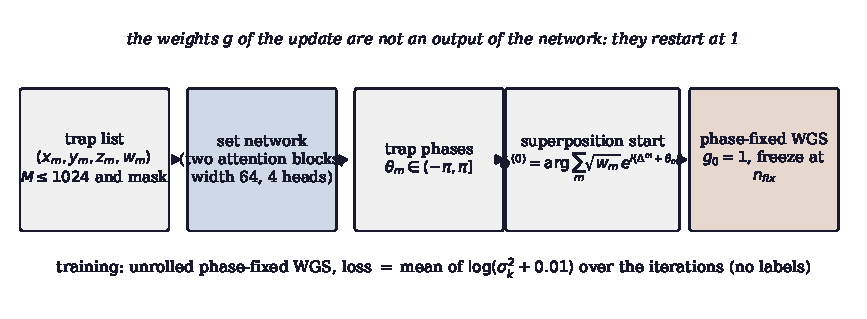
\includegraphics[width=\textwidth]{fig-method.pdf}
\caption{The learned warm start: a trap list of at most 1024 traps with a mask enters a permutation-equivariant set network that predicts one phase per trap; the superposition hologram built from those phases starts phase-fixed WGS, whose weights restart at one; training minimizes the log spread along an unrolled copy of the iteration, without labels.}
\label{fig:method}
\end{figure}

\subsection{The start hologram}\label{sec:start}

Given predicted phases $\theta_m$, the SLM start is the superposition of the single-trap holograms with those phases, the form of the SR hologram of~\cite{dileonardo} with learned instead of random phases:
\begin{equation}
\phi^{(0)}_j=\arg\sum_{m=1}^{M}a_m\,e^{\,i(\Delta_j^m+\theta_m)},\qquad a_m=\sqrt{w_m}.
\label{eq:start}
\end{equation}
This is the back-projection of the coefficients $a_me^{i\theta_m}$ of Section~\ref{sec:forward}, and it is the same operation the random start performs with $\theta_m$ drawn from the portable random generator of the engine. The start field is $V^{(0)}_m=V_m(\phi^{(0)})$ from Eq.~\eqref{eq:forward}. When the traps are well separated
the cross terms between traps are small and $\arg V^{(0)}_m\approx\theta_m$, so $\theta_m$ is, to a first approximation, the phase the iteration sees at trap $m$ in its first step. When the traps are dense the cross terms are not small, and $\arg V^{(0)}_m$ differs from $\theta_m$; this is the case of every geometry in the held-out set (at least 40 traps).

The start hologram is the only place where the network output meets the engine, and its form was chosen so that a network that predicts the right phases reproduces exactly what a converged run would hold: the phases of the converged field at the traps, back-projected with the target amplitudes. The same function builds the oracle start of Section~\ref{sec:oracle-design}, with the phases of a converged run in place of the network phases, so that the two starts differ only in where the phases come from and the comparison is not confounded by a different construction of the hologram.

\subsection{The iteration the start enters}\label{sec:m07}

Phase-fixed WGS keeps one weight $g_{k,m}$ per trap and one focal phase $\psi_{k,m}$ per trap. With $B_{k}(m)=|V^{(k)}_m|/a_m$ the trap amplitude relative to its target, the iteration for $k\ge1$ is
\begin{align}
g_{1,m}&=1,\qquad g_{k,m}=g_{k-1,m}\,\frac{\langle B_{k-1}\rangle}{B_{k-1}(m)}\quad(k\ge2),\label{eq:weights}\\
\psi_{k,m}&=\arg V^{(k-1)}_m\ \ (k\le\nfix),\qquad \psi_{k,m}=\psi_{\nfix,m}\ \ (k>\nfix),\label{eq:freeze}\\
\phi^{(k)}_j&=\arg\sum_{m=1}^{M}g_{k,m}\,a_m\,e^{\,i(\psi_{k,m}+\Delta_j^m)},\label{eq:update}
\end{align}
where $\langle\cdot\rangle$ is the mean over the traps and $\nfix$ the freeze index; the engine default of the product is $\nfix=12$ after Kim et al.~\cite{kim2019}. The weights update multiplicatively and carry the memory of all earlier corrections; the focal phase follows the field for the first $\nfix$ iterations and is then fixed, which removes the focal-phase perturbation that
re-imposing the laser amplitude at the SLM would otherwise introduce. The start enters in one place only: the field $V^{(0)}$ of Eq.~\eqref{eq:start}, which gives the phases $\psi_{1}=\arg V^{(0)}$ of the first iteration. The weights restart at one whatever the start is. The relative amplitude $B_k$ is the field amplitude $|V_m|$ divided by the target amplitude $a_m$, as in weighted GS~\cite{dileonardo}. This is the structural fact on which the theory of Section~\ref{sec:theory} rests: a warm start can only change the iteration through the phases of the first $\nfix$
steps.

\subsection{The network}\label{sec:network}

The network is a permutation-equivariant set transformer over the trap list (Set Transformer~\cite{settransformer}, Deep Sets~\cite{deepsets}). Each trap $m$ is described by its position in focal bins $(\hat x_m,\hat y_m)=(x_m,y_m)/128$, its depth in Rayleigh ranges $\hat z_m=z_m/(4z_{\mathrm R})$ and its weight, and receives a vector of $29$ features: the normalized coordinates, $\hat z_m$, $w_m-1$, $\varrho_m^2=\hat x_m^2+\hat y_m^2$, and Fourier features of the position at six octaves~\cite{fourierfeatures},
\begin{equation}
\mathbf f_m=\big[\hat x_m,\hat y_m,\hat z_m,w_m-1,\varrho_m^2,\ \sin(\pi\nu\hat x_m),\cos(\pi\nu\hat x_m),\sin(\pi\nu\hat y_m),\cos(\pi\nu\hat y_m)\big]_{\nu\in\{1,2,4,8,16,32\}}.
\label{eq:features}
\end{equation}
Two layers embed $\mathbf f_m$ to width $d=64$. Two blocks of attention follow, each with $4$ heads of width $16$, a residual connection, and a feed-forward layer of width $128$, with the padded traps removed by an additive bias of $-10^{4}$ on the attention logits:
\begin{equation}
\mathbf h\leftarrow\mathbf h+W_o\,\mathrm{softmax}\!\Big(\frac{QK^{\top}}{\sqrt{d_h}}+\mathbf b\Big)V,\qquad \mathbf h\leftarrow\mathbf h+W_2\,\mathrm{ReLU}(W_1\mathbf h),\qquad b_{jm}=-10^4\,(1-\mathrm{mask}_m),
\label{eq:attention}
\end{equation}
where $Q,K,V$ are linear maps of $\mathbf h$ and $d_h=16$; the output projections $W_o$ and $W_2$ start at zero so that the untrained network is the embedding alone. No layer normalization is used, so that the exported graph contains only operators that a browser inference runtime provides. With $\bar{\mathbf h}$ the mean of $\mathbf h$ over the valid traps, the predicted phase of trap $m$ is
\begin{equation}
\theta_m=\mathrm{wrap}\Big(\mathrm{MLP}\big([\mathbf h_m,\bar{\mathbf h}]\big)+\big(c_0+20\,\mathbf w_c^{\top}\bar{\mathbf h}\big)\,\varrho_m^2\Big),\qquad \mathrm{wrap}(t)=\operatorname{atan2}(\sin t,\cos t),
\label{eq:output}
\end{equation}
where the second term is a set-dependent quadratic (Fresnel-like) phase law with a learned scalar $c_0$ (initialized at $80$) and a learned vector $\mathbf w_c$; it lets the network write the chirp that a regular array's converged phases follow without having to represent hundreds of radians with an MLP. The network has $\nParams$ parameters and its ONNX export holds $\onnxBytes$ bytes. The value of $c_0$ after training is the initial one to
within a fraction of a percent, so the learned part is the correction on top of the chirp.

\subsection{Training without labels}\label{sec:training}

Converged WGS phases are not unique: the global phase is free and the many fixed points of the iteration give different phases for the same geometry, so a regression onto converged phases would have an ambiguous target. We train instead through the iteration. A differentiable copy of Eqs.~\eqref{eq:weights}--\eqref{eq:update} (separable point-trap form in single precision, checked against the engine's phase-fixed WGS in the repository's tests) is
unrolled for $K=10$ iterations from the start of Eq.~\eqref{eq:start}, and the loss is the weighted mean of the log of the squared spread:
\begin{equation}
\mathcal L(\vartheta)=\frac{1}{\sum_{k=0}^{K}\omega_k}\sum_{k=0}^{K}\omega_k\ \mathbb E_{\mathcal T\sim\mathcal D}\Big[\log\big(\relstd_k^2+0.01\big)\Big],\qquad \omega_0=0.3,\ \omega_{k\ge1}=1,
\label{eq:loss}
\end{equation}
with $\relstd_k$ the spread (in percent) after unrolled iteration $k$ and $\relstd_0$ that of the start. The constant $0.01$ saturates the loss below a spread of 0.1 percent, so that the network is not rewarded for precision the iteration reaches by itself; the log compresses the large spreads of the first iterations. The unrolled iteration uses the freeze index $\nfix=3$, chosen because an earlier trial at
$\nfix=12$ with 14 unrolled iterations produced a start that reached about the random level. The global phase is invariant by construction because the loss reads intensities only. The trap sets are drawn on the fly from seeded generators: square and hexagonal lattices, rings with an optional concentric ring, random sets with a minimum spacing, stacks of two to four planes and random three-dimensional sets, with the proportions
$0.25$, $0.15$, $0.15$, $0.2$, $0.15$, $0.1$, optional position jitter and random weights in $[0.5,2]$ for 30 percent of the sets; sets of fewer than 40 traps are discarded with probability $0.6$ because a sparse array reaches 1 percent at the first iteration from any start. The generators contain no quasi-periodic family, so the benchmark geometry of that kind is unseen.

\subsection{Algorithms and parameters}\label{sec:algorithm}

Algorithm~\ref{alg:warm} is the method as run by the engine; Algorithm~\ref{alg:train} is the offline training. The inference algorithm has two branches that matter for the interpretation of every measurement below: when a network is released the phases come from it, and when none is released the phases are drawn from the seeded generator, so that the same function answers in both cases and the baseline is not a different code path. The training algorithm sees only trap sets and the differentiable iteration; it never reads a held-out geometry and never reads a converged phase, which is what makes it unsupervised in the sense of the problem statement.

\begin{algorithm}[t]
\caption{Learned warm start for phase-fixed WGS (inference and run).}\label{alg:warm}
\begin{algorithmic}[1]
\Require trap set $\mathcal T=\{(x_m,y_m,z_m,w_m)\}$, network $g_\vartheta$ (or none), freeze index $\nfix$, budget $K_{\max}$, seed
\Ensure SLM phase $\phi^{(K)}$ and the history $\relstd(\phi^{(k)})$
\State convert $\mathcal T$ to bins and Rayleigh ranges, pad to $1024$ traps with a mask
\If{a network is released} $\theta\gets g_\vartheta(\mathcal T)$ \Else{} $\theta_m\sim U[0,2\pi)$ from the seeded generator \EndIf
\State $\phi^{(0)}\gets\arg\sum_ma_me^{i(\Delta^m+\theta_m)}$ \Comment{Eq.~\eqref{eq:start}}
\State $V^{(0)}\gets$ project$(\phi^{(0)})$;\quad $g_1\gets\mathbf 1$
\For{$k=1,\dots,K_{\max}$}
  \If{$k\ge2$} $g_k\gets g_{k-1}\langle B_{k-1}\rangle/B_{k-1}$ \EndIf \Comment{Eq.~\eqref{eq:weights}}
  \State $\psi_k\gets\arg V^{(k-1)}$ if $k\le\nfix$, else $\psi_{\nfix}$ \Comment{Eq.~\eqref{eq:freeze}}
  \State $\phi^{(k)}\gets\arg\sum_mg_{k,m}a_me^{i(\psi_{k,m}+\Delta^m)}$;\quad $V^{(k)}\gets$ project$(\phi^{(k)})$ \Comment{Eq.~\eqref{eq:update}}
\EndFor
\State \Return $\phi^{(K_{\max})}$ and the history of $\relstd$, $\eta$, $u$
\end{algorithmic}
\end{algorithm}

\begin{algorithm}[t]
\caption{Unsupervised training of the warm-start network through the unrolled iteration.}\label{alg:train}
\begin{algorithmic}[1]
\Require generator of trap sets $\mathcal D$ with a seed, steps $T$, batch $B$, unroll $K$, freeze index $\nfix$
\State initialize $\vartheta$ from the initialization seed; AdamW with a warm-up and a cosine schedule
\For{$t=1,\dots,T$}
  \State draw $B$ trap sets, pad and mask;\quad $\theta\gets g_\vartheta(\mathcal T)$
  \State run the unrolled iteration for $K$ steps from the start of Eq.~\eqref{eq:start}, recording $\relstd_0,\dots,\relstd_K$
  \State $\mathcal L\gets$ Eq.~\eqref{eq:loss};\quad clip the gradient norm to $1$;\quad update $\vartheta$
\EndFor
\State \Return $\vartheta$ \Comment{evaluated on held-out geometries before any release}
\end{algorithmic}
\end{algorithm}

Table~\ref{tab:params} lists every parameter of the method with its value and where the value comes from. Values that are choices of the product, not of a source, are marked as such. The architecture was sized to the limit the product sets for a model that a browser must download and run, at most 1 MB as an exported graph, and the training budget to what a single laptop GPU delivers in under two hours; neither was tuned against the held-out set, which training never reads. The freeze index of the training unroll, $\nfix=3$, is the one parameter that departs from the published default, and it is the parameter that the ablation of Section~\ref{sec:ablation} isolates.

\begin{table}[t]
\centering\small
\begin{tabular}{@{}lll@{}}
\toprule
Parameter & Value & Origin \\
\midrule
width $d$, layers, heads, feed-forward & 64, 2, 4, 128 & choice of the product, sized to stay under 1 MB \\
Fourier octaves $\nu$ & 1, 2, 4, 8, 16, 32 & choice of the product after~\cite{fourierfeatures} \\
maximum number of traps & 1024 & contract of the model slot \\
unroll $K$, freeze index in training & 10, 3 & choice of the product (Section~\ref{sec:training}) \\
loss constants $0.01$, $\omega_0$ & 0.01, 0.3 & choice of the product \\
steps, batch, peak learning rate & 6000, 8, $8\times10^{-4}$ & choice of the product (AdamW~\cite{adamw}, decay $10^{-5}$) \\
data seed, initialization seed & 20261101, 7 & recorded in the training configuration \\
freeze index of the engine default $\nfix$ & 12 & Kim et al.~\cite{kim2019} \\
iteration budget $K_{\max}$ & \budget & evaluation protocol (Section~\ref{sec:design}) \\
\bottomrule
\end{tabular}
\caption{Parameters of the learned warm start and of the iteration it feeds, with their origin; the network and training values are those of the trained candidate whose configuration is recorded with its checkpoint.}
\label{tab:params}
\end{table}

\subsection{Complexity and implementation}\label{sec:complexity}

The attention of a block over $M$ traps costs $M^2d$ multiply-adds for $QK^\top$ and the same for the weighted sum, that is $2M^2d$ per block, so inference is $O(LM^2d)$ for $L$ blocks, plus $O(Md^2)$ for the linear layers; the full attention is quadratic in the number of traps, not linear. Counting the multiply-adds of the attention products and of one iteration of the point form of phase-fixed WGS (a projection and a back-projection, each a separable product of $N^2M$ terms),
\begin{equation}
C_{\mathrm{net}}\approx 2\,L\,M^{2}d,\qquad C_{\mathrm{iter}}\approx 2\,N^{2}M,
\label{eq:cost}
\end{equation}
which at the maximum of $M=1024$ traps, $L=2$, $d=64$ and $N=256$ give about $2.7\times10^{8}$ and $1.3\times10^{8}$ multiply-adds, so by operation count the network pass at the largest array is of the order of two iterations of the method it is meant to shorten. The start hologram of Eq.~\eqref{eq:start} costs one back-projection, as one iteration does. Training is offline and local, on one GPU, never in the continuous
integration of the product.

The method is implemented in the engine of the product as the module \texttt{methods/learned/b3\_warm\_start.py} (the method), \texttt{learned/nets.py} (the network), \texttt{learned/torch\_forward.py} (the differentiable iteration), \texttt{learned/training.py} (Algorithm~\ref{alg:train}) and \texttt{learned/heldout.py} and \texttt{learned/evaluation.py} (the held-out sets and the evaluation of Section~\ref{sec:design}). With no released network, the module answers with the iteration from its own random start and marks the result as a baseline, so that
a missing model is never mistaken for a learned one.

\section{Theory: what a start can and cannot change}\label{sec:theory}

The propositions of this section are exact statements about the iteration of Section~\ref{sec:m07} and the network of Section~\ref{sec:network}; the relation of Section~\ref{sec:conjecture} is a conjecture with the evidence for it. Together they say where a warm start can act and why the gain it can give is bounded by the freeze index.

\subsection{Invariances}\label{sec:invariance}

\begin{proposition}[global phase]\label{prop:global}
Let $c\in\mathbb R$ and let the start phases be shifted, $\theta'_m=\theta_m+c$ for all $m$. Then for every $k\ge0$ the holograms satisfy $\phi'^{(k)}=\phi^{(k)}+c$ and the fields $V'^{(k)}=e^{ic}V^{(k)}$, so $\relstd_k$, $\eta_k$ and $u_k$ are the same sequences.
\end{proposition}
\begin{proof}
For $k=0$, Eq.~\eqref{eq:start} gives $\phi'^{(0)}=\arg\big(e^{ic}\sum_ma_me^{i(\Delta^m+\theta_m)}\big)=\phi^{(0)}+c$, and Eq.~\eqref{eq:forward} gives $V'^{(0)}_m=N^{-2}\sum_jA_je^{i(\phi^{(0)}_j+c-\Delta_j^m)}=e^{ic}V^{(0)}_m$. Assume the claim for $k-1$. The relative amplitudes $B_{k-1}(m)=|V^{(k-1)}_m|/a_m$ do not change, so the weights of Eq.~\eqref{eq:weights} do not change; the phases of Eq.~\eqref{eq:freeze} become $\psi'_{k,m}=\psi_{k,m}+c$ (and the frozen
phase $\psi'_{\nfix}=\psi_{\nfix}+c$). Eq.~\eqref{eq:update} then gives $\phi'^{(k)}=\phi^{(k)}+c$, and Eq.~\eqref{eq:forward} gives $V'^{(k)}=e^{ic}V^{(k)}$. The intensities are unchanged. \end{proof}

Proposition~\ref{prop:global} is why the loss of Eq.~\eqref{eq:loss}, which reads intensities only, needs no special treatment of the global phase, and why a regression onto converged phases would need one.

\begin{proposition}[permutation equivariance]\label{prop:equivariance}
Let $\pi$ be a permutation of the valid traps and $\pi\mathcal T$ the permuted trap set. The network of Eqs.~\eqref{eq:features}--\eqref{eq:output} satisfies $g_\vartheta(\pi\mathcal T)=\pi\,g_\vartheta(\mathcal T)$, and the start hologram of Eq.~\eqref{eq:start} is the same for $\mathcal T$ and $\pi\mathcal T$.
\end{proposition}
\begin{proof}
The features of Eq.~\eqref{eq:features} and the embedding act on each trap separately, so they commute with $\pi$. In Eq.~\eqref{eq:attention} the queries are permuted with the traps; the logits of query $m$ over the keys are permuted with the keys, and the softmax and the weighted sum of the values are invariant to a permutation of the keys, so the output for trap $m$ is unchanged; the additive mask follows its trap.
The mean $\bar{\mathbf h}$ over the valid traps is invariant to $\pi$, and the readout of Eq.~\eqref{eq:output} acts row by row with $\bar{\mathbf h}$ and $\varrho_m^2$ attached to trap $m$. Hence $\theta_m$ follows trap $m$. The sum of Eq.~\eqref{eq:start} runs over all traps and does not depend on their order. \end{proof}

The network has no positional index of any kind, so the order in which a user lists the traps cannot change the start, and the padded entries (removed by the mask) cannot change it either. The proposition is also the reason for a set network and against a recurrent or convolutional one: an ordering of traps would be an arbitrary input that the network would have to learn to ignore.

\subsection{What the start changes}\label{sec:start-change}

\begin{proposition}[the start enters through the frozen phase]\label{prop:washout}
(a) For $\nfix=1$, every hologram $\phi^{(k)}$, $k\ge1$, is a function of the trap set and of the vector $\psi_1=\arg V^{(0)}$ alone. (b) For general $\nfix$, every $\phi^{(k)}$ with $k\ge\nfix$ is a function of the trap set and of the trajectory $V^{(0)},\dots,V^{(\nfix-1)}$, that is, of the start through $\nfix-1$ applications of Eqs.~\eqref{eq:weights}--\eqref{eq:update}.
\end{proposition}
\begin{proof}
(a) With $\nfix=1$ Eq.~\eqref{eq:freeze} gives $\psi_{k}=\psi_1$ for all $k\ge1$ and $g_1=\mathbf 1$, so $\phi^{(1)}=\arg\sum_ma_me^{i(\psi_1+\Delta^m)}$ depends on $\psi_1$ only. Then $V^{(1)}$ is a function of $\phi^{(1)}$, $g_2$ of $V^{(1)}$ by Eq.~\eqref{eq:weights}, and $\phi^{(2)}=\arg\sum_mg_{2,m}a_me^{i(\psi_1+\Delta^m)}$ of $g_2$ and $\psi_1$; the induction continues. (b) The frozen phase is $\psi_{\nfix}=\arg V^{(\nfix-1)}$ by Eq.~\eqref{eq:freeze}, and the weights $g_k$ for $k\le\nfix$ are functions of $V^{(1)},\dots,V^{(\nfix-1)}$ by Eq.~\eqref{eq:weights}; after the freeze the sequence is generated by the same two rules from these quantities, so the start enters only
through the trajectory up to $V^{(\nfix-1)}$. \end{proof}

Part (a) turns the warm-start problem at $\nfix=1$ into the prediction of $M$ phases and nothing else: the network's $\theta_m$ become, to the extent that the cross terms of Eq.~\eqref{eq:start} are small, the frozen phases of the whole run. Part (b) holds for any deterministic iteration and constrains nothing by itself; its content here is that the start enters only through $V^{(0)}$ while the weights restart at one, so at the engine default $\nfix=12$ the start has to survive eleven applications of the iteration to matter. Whether it does is a property of the dynamics of the iteration, not of the network, and it is measured in Section~\ref{sec:ablation}: from the phases of a converged
run (the best start one could hope to predict) the iteration at $\nfix=12$ still needs \OTwelveMed{} iterations (median over ten geometries) against \ORMed{} from a random start.

\subsection{An accounting bound on the weights}\label{sec:weights-bound}

The weights restart at one whatever the start is, so a warm start does not transfer the correction that a converged run has stored in $g$. How long the weights need to rebuild it is bounded below by an accounting identity. Let $S_k=\max_m\log g_{k,m}-\min_m\log g_{k,m}$ be the log-spread of the weights after iteration $k$, and
$s_k=\log\big(\max_mB_{k-1}(m)/\min_mB_{k-1}(m)\big)$ the allowance of the update at iteration $k\ge2$.

\begin{proposition}[allowance]\label{prop:allowance}
For every run and every $k\ge2$,
\begin{equation}
S_k\ \le\ \sum_{j=2}^{k}s_j .
\label{eq:allowance}
\end{equation}
\end{proposition}
\begin{proof}
By Eq.~\eqref{eq:weights}, $\log g_{k,m}=\log g_{k-1,m}+\log\langle B_{k-1}\rangle-\log B_{k-1}(m)$. The term $\log\langle B_{k-1}\rangle$ is common to all traps and cancels in the spread. The spread of a sum is at most the sum of the spreads, and the spread of $-\log B_{k-1}(m)$ over $m$ is $s_k$. Hence $S_k\le S_{k-1}+s_k$, and $S_1=0$ since $g_1=\mathbf 1$. \end{proof}

If a converged run holds a weight spread $S^\star$, no run that starts from $g=\mathbf 1$ reaches that spread before the iteration $k_{\mathrm{floor}}=\min\{k:\sum_{j=2}^ks_j\ge S^\star\}$. The bound is a statement about the restart; its tightness is measured, not assumed: we compute $S_k$ and the allowance along the runs of Section~\ref{sec:ablation} and compare $k_{\mathrm{floor}}$ with the iterations to 1 percent (Table~\ref{tab:weights}).

\subsection{A relation between the freeze index and the iterations}\label{sec:conjecture}

\begin{conjecture}[iterations follow the freeze]\label{conj:freeze}
For the random start and the network start on dense arrays (at least 40 traps) for which the iteration reaches 1 percent, the number of iterations to 1 percent is the freeze index plus a short tail, $k_1=\nfix+t$ with $t$ of the order of one to four iterations on most geometries, and the start changes $t$ and the probability of reaching 1 percent. The relation is a description of the starts tried here and has counterexamples, listed below.
\end{conjecture}

We do not prove the conjecture; the evidence is of four kinds, all in Section~\ref{sec:ablation}. (i) Before the freeze the spread of the default run stays at several percent: the median trajectory of the random start at $\nfix=12$ is \trRTwelveEleven{} percent at iteration 11 and \trRTwelveTwelve{} percent at 12, and drops to \trRTwelveThirteen{} percent at 13, the first iteration that uses the frozen phase. (ii) The sweep of the freeze index
puts the median $k_1$ of the random start at \swTwelveEx, \swEightEx, \swSixEx, \swFourEx{} and \swThreeEx{} iterations above the freeze index for $\nfix=12,8,6,4,3$; these medians include the runs that reach the cap of the budget (\swThreeNever{} percent of the runs at $\nfix=3$ and \swFourNever{} percent at $\nfix=4$), and the excess of the runs that converge alone was not computed, because the sweep stores medians and not the count of each run, so the tail of one to four is exceeded at $\nfix=3$ and is not verified on converged runs. (iii) The network start at $\nfix=12$ has the same median as the random start, and (iv) the phases of a converged run lower the median at $\nfix=12$ by \OTwelveGain{} iteration only. The counterexamples are in Table~\ref{tab:oracle}: the random start reaches 1 percent before the freeze index at $\nfix=12$ on one of the ten geometries (\texttt{gen/09}), the converged phases do so on three (\texttt{gen/00}, \texttt{gen/07} and \texttt{gen/09}), and at $\nfix=3$ the converged phases lower the median from \ORThreeMed{} to \OThreeMed{} iterations and converge on three geometries where the random start never does. These are ten geometries and one seed. The conditions under which the relation fails are also in the data: a freeze that is too early locks phases that are
incompatible with a uniform solution, and then the run never reaches 1 percent; the share of such runs rises as the freeze index falls (Table~\ref{tab:sweep}). A warm start can therefore act on the second term, on the share of runs that converge, and on the final spread, and could lower the first term only by lowering the index at which freezing is safe.

\subsection{Consequences for the experiment}\label{sec:consequences}

The propositions fix what the experiments must separate. Because the iteration depends on the start only through $\psi_{\nfix}$ (Proposition~\ref{prop:washout}), a network start and a change of $\nfix$ are two different handles on the same quantity, and an experiment that changes both at once cannot attribute the effect: the candidate network was trained and first evaluated at $\nfix=3$ while its baseline ran at the default $\nfix=12$. The ablation of Section~\ref{sec:ablation} therefore crosses the two factors, and the sweep of $\nfix$ with
and without the network tests Proposition~\ref{prop:washout}(a) directly at $\nfix=1$. A fair comparison of a learned start therefore needs the baseline at the same freeze index as the candidate, in addition to the baseline at the published default: the first isolates the contribution of the network, the second measures the practical gain over the method as published. The first evaluation of the candidate compared it only with the second, and the difference between the two comparisons is the result of this paper. Proposition~\ref{prop:allowance} gives a check that costs nothing: the weights cannot be the binding constraint if $k_{\mathrm{floor}}$ is far below the measured iterations.

\section{Experimental design}\label{sec:design}

\subsection{Hypotheses}\label{sec:hypotheses}

Three hypotheses were fixed, with their thresholds, before the network was trained, and a fourth was added after the first evaluation to explain its outcome; we label it as such.
\begin{description}
\item[H1 (speed).] On geometries held out from training, the median number of iterations to 1 percent, $k_1$ of Eq.~\eqref{eq:k1}, of phase-fixed WGS from the network start is at most half that from the random start: the ratio of the medians is at least $2$.
\item[H2 (accuracy).] The final efficiency and the final uniformity of the run from the network start differ from those of the random start by at most 1 percent (relative difference of the medians).
\item[H3 (size).] The exported network is at most 1 MB as an ONNX graph. Its inference time in a browser (a threshold of 10 ms in the product's research record) belongs to the same acceptance test; it was not measured here because H1 failed first.
\item[H4 (attribution; added after the first evaluation).] If the network start shortens the iteration, the gain is not reproduced by a random start with the same freeze index $\nfix$; if instead a random start with the same $\nfix$ reproduces it, the gain belongs to the freeze index. The prediction of the second reading, which Section~\ref{sec:theory} motivates, is that a network start at the default $\nfix=12$ shows no gain, and that the gain of the candidate at $\nfix=3$ is the gain of $\nfix=3$.
\end{description}
H1 and H2 are the acceptance test of the model slot of the product: a network that fails either is not released. H3 is met by the candidate. H4 is exploratory; its tests are the ablation of Section~\ref{sec:ablation}, and it does not change the status of H1 and H2.

\subsection{Data and provenance}\label{sec:data}

The held-out file was written once, before any training run, from seeded generators, and is identified by its sha256 digest (checked by the measurement script against the digest recorded with the rejected candidate). Training reads other seeds and never this file. Table~\ref{tab:heldout} describes it. Its $\nGen$ generated trap sets come from the same generators as the training data (lattices, hexagonal lattices, rings, random sets with a minimum spacing and three-dimensional
stacks) with a fresh seed, and are filtered to be demanding: at least 40 traps and a random-start phase-fixed WGS run, on a selection seed that is not an evaluation seed, that needs more than 3 iterations to reach 1 percent. A sparse array reaches 1 percent at the first iteration from any start, so it cannot show a warm start, and the filter looks only at the baseline, never at a model. The remaining $\nBench$ geometries are the six point-trap geometries of
the benchmark of the product (G1 to G6: a $10	imes10$ square lattice, a ring of 36 traps, 100 random traps, a quasi-periodic array of 119 traps, a three-dimensional lattice of $5	imes5	imes3$ traps and a $32	imes32$ lattice of 1024 traps), on the grids of the benchmark, the last of which is $512^2$ pixels. The quasi-periodic benchmark geometry belongs to a family absent from training. The generated sets have between \trapsMin{} and \trapsMax{} traps (median \trapsMed). The engine setup of the generated sets is an SLM of $\nPixGen\times\nPixGen$ pixels of pitch \pitchUm{} $\mu$m with a zero padding of \padGen, a lens of \focalMm{} mm and a wavelength of \lambdaNm{} nm.

\begin{table}[t]
\centering\small
\resizebox{\textwidth}{!}{\begin{tabular}{@{}lrrll@{}}
\toprule
Group & Geometries & Traps & Grid & Origin \\
\midrule
generated, demanding & \nGen & \trapsMin--\trapsMax & $\nPixGen^2$, pad \padGen & fresh seed; at least 40 traps; the random start needs more than 3 iterations \\
benchmark G1 to G6 & \nBench & 36--\benchTrapsMax & $256^2$ and $512^2$ & benchmark geometry records of the product \\
\bottomrule
\end{tabular}}
\caption{Composition of the held-out set of $\nGeo$ trap geometries: the generated geometries are filtered to be demanding for the baseline, and the benchmark geometries are those of the product's benchmark; neither group is used in training.}
\label{tab:heldout}
\end{table}

\subsection{Methods compared}\label{sec:compared}

Every method is run by the engine of the product on the same geometries, seeds and budget; no number is taken from a publication. The published method is phase-fixed WGS of Kim et al.~\cite{kim2019} at its default freeze index $\nfix=12$ from the random superposition start of~\cite{dileonardo}. Two published iterations that precede it serve as references: the Gerchberg--Saxton iteration~\cite{gs1972} and weighted GS~\cite{dileonardo}, both from the random start. The proposed
method is phase-fixed WGS from the network start. The ablation adds the arms that separate the two factors that the candidate changed at once, the start and the freeze index:
\begin{itemize}
\item random start, $\nfix=12$ (the published default);
\item random start, $\nfix=3$ (the early freeze alone, no network);
\item network start, $\nfix=12$ (the network alone, the published freeze);
\item network start, $\nfix=3$ (the candidate as it was trained and first evaluated).
\end{itemize}
A sweep of $\nfix$ over $1,2,3,4,6,8$ and $12$ for both starts (on every second generated geometry, $30$ of them) and an oracle start (Section~\ref{sec:oracle-design}) complete the design. The network is the trained candidate: the checkpoint at the last of its $\trainSteps$ steps, read from the training directory of the data root; nothing is retrained.

\subsection{Metrics and statistics}\label{sec:stats}

The per-run quantities are those of Eqs.~\eqref{eq:metrics} and~\eqref{eq:k1}, read after each iteration by the engine. For a geometry $g$ and an arm the per-geometry value is the median over the $\nSeeds$ seeds,
\begin{equation}
\tilde k_g=\operatorname{median}_{s\in\{301,302,303\}}\,k_1^{(g,s)},
\label{eq:pergeo}
\end{equation}
and the summary of an arm is the median over geometries, $\tilde k=\operatorname{median}_g\tilde k_g$; the ratio of two arms is the ratio of their summaries, $\rho=\tilde k_{\mathrm{ref}}/\tilde k_{\mathrm{arm}}$. The same seed gives the same random phases in every arm, so the arms are paired by geometry and seed. The uncertainty of $\tilde k$ and of $\rho$ is a percentile bootstrap over geometries,
\begin{equation}
\mathrm{CI}_{95}=\big[\,q_{2.5}\{\tilde k^{*b}\}_{b=1}^{B},\ q_{97.5}\{\tilde k^{*b}\}_{b=1}^{B}\,\big],\qquad B=10^{4},
\label{eq:boot}
\end{equation}
where $\tilde k^{*b}$ is the summary of the $b$-th resample of the $\nGeo$ geometries with replacement~\cite{efron}, with a fixed seed for the resampling. Because $k_1$ is an integer capped at $\budget+1$ and the arms differ in how many runs hit the cap, we also report the share of runs that never reach 1 percent, the quartiles of $\tilde k_g$ and the median final $\relstd$. The difference between two arms on the geometries is tested with the exact two-sided sign test on the paired $\tilde k_g$, ties dropped,
\begin{equation}
p=\min\Big\{1,\ 2\sum_{j=0}^{\min(n_+,n_-)}\binom{n_++n_-}{j}2^{-(n_++n_-)}\Big\},
\label{eq:sign}
\end{equation}
with $n_+$ and $n_-$ the numbers of geometries where the first arm needs more and fewer iterations. The sign test uses no distributional assumption and is robust to the heavy tail of the capped counts. Final-efficiency differences are the relative difference of the medians over geometries, as in the acceptance test.

\subsection{Oracle start and weight accounting}\label{sec:oracle-design}

Two further measurements probe the theory. The oracle start is the best start a predictor could hope for: the phases $\arg V_m$ of the final field of a random-start phase-fixed WGS run of $\budget$ iterations on the same geometry and seed are used as the trap phases $\theta_m$ of Eq.~\eqref{eq:start}, and the iteration is run again from there with $\nfix=12$, $3$ and $1$. It is computed on the first ten generated geometries with the first seed. The weight accounting runs the iteration with a wrapper that records $S_k$ and $s_k$ of Section~\ref{sec:weights-bound} at every iteration, from the random start and from the oracle start, for $\nfix=12$ and $\nfix=3$, on the same ten geometries and seed, and checks Eq.~\eqref{eq:allowance} on every run.

The two probes answer different questions. The oracle start bounds what any predictor of trap phases could gain at a given freeze index, and its comparison with the network start tells whether the network is far from that bound or the bound itself is small. The accounting tests a specific explanation of the bound, that the restart of the weights limits the iteration, by comparing the lower bound it implies with the iterations that the run actually needs. Both are exploratory and are reported with their small samples.

\subsection{Hardware and run times}\label{sec:hardware}

The engine is the NumPy implementation of the product (the point-trap form for every geometry); the network runs in PyTorch on the CPU for the inference of each geometry, and the measurement of all arms was run with \nWorkers{} worker processes on the development workstation (Intel Core i9-14900HX, 48 GB of RAM), in \runtimeMin{} minutes of wall-clock time. The network was trained on a single RTX 4070 Laptop GPU in \trainMinutes{} minutes. The generated trap sets and the held-out file do not depend on the machine; the wall-clock numbers do, and none of the conclusions rests on a time. The number of worker processes does not change any result, because each run is a pure function of its geometry, seed, start and freeze index, and the results are gathered by identifier. The measurement script checks the held-out digest before it starts and stops if it differs. Every random choice goes through the portable seeded generator of the engine, so a rerun reproduces the same numbers up to the floating point of the machine's fast Fourier transform.

\section{Results}\label{sec:results}

\subsection{Training behaviour}\label{sec:res-training}

The network trained for $\trainSteps$ steps. The loss of Eq.~\eqref{eq:loss} fell from \trainFirstLoss{} at the first logged step to an average of \trainLastLoss{} over the last ten logged steps (Figure~\ref{fig:training}a), a decrease that the batch-to-batch variation of the trap sets makes noisy: the batches differ in the number of traps from one step to the next. The logged quantity that matters for the question is the spread after the last unrolled iteration, which the training script measures for the network
phases and, on the same batch, for random phases (Figure~\ref{fig:training}b). Over the last twenty logged steps the median spread after ten iterations is \trainSigNet{} percent for the network phases and \trainSigRand{} percent for random phases at the training freeze index $\nfix=3$: the network is not better than random phases at the end of the unrolled iteration on the training distribution, although it is better at the first iteration (\trainSigNetFirst{} against \trainSigRandFirst{} percent after iteration 1).
The advantage the loss rewards at the start is gone by iteration ten. On the held-out geometries the advantage after the first iteration is absent as well: the median spread after iteration 1 is \trNThreeOne{} percent for the network start and \trRTwelveOne{} percent for the random start (Table~\ref{tab:main} gives the other quantities).

\begin{figure}[t]
\centering
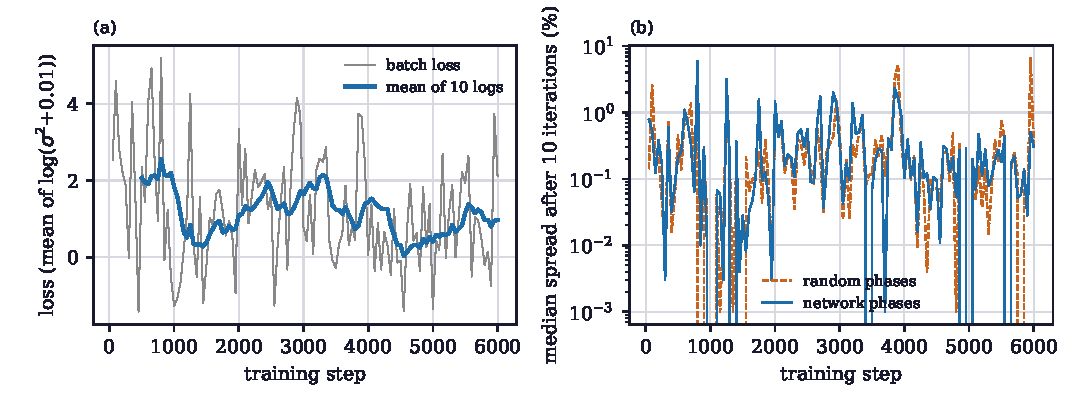
\includegraphics[width=\textwidth]{fig-training.pdf}
\caption{Training of the warm-start network: (a) loss of Eq.~\eqref{eq:loss} per logged step with a mean of ten logs; (b) median spread after the last unrolled iteration for the network phases and for random phases on the same training batches, per logged step, on a logarithmic axis.}
\label{fig:training}
\end{figure}

\subsection{Main comparison on held-out geometries}\label{sec:res-main}

Table~\ref{tab:main} gives the four phase-fixed WGS arms and the two published references on the $\nGeo$ held-out geometries ($\nSeeds$ seeds each, a budget of $\budget$ iterations). The published default (random start, $\nfix=12$) reaches 1 percent at a median of \itRTwelve{} iterations, with a tight spread (quartiles \itRTwelveQa{} to \itRTwelveQb) and \neverRTwelve{} percent of runs that do not reach it within the budget; the references are
slower or less reliable: the unweighted Gerchberg--Saxton iteration does not reach 1 percent within the budget on \neverMFour{} percent of the runs, and weighted GS reaches it at a median of \itMSix{} iterations (interval \itMSixLo{} to \itMSixHi), failing on \neverMSix{} percent of the runs. The candidate, the network start at $\nfix=3$, reaches 1 percent at a median of \itNThree{} iterations, with a 95\% bootstrap interval of \itNThreeLo{} to \itNThreeHi{}, and the ratio of the default's median to the candidate's is \ratioRoverN{} (interval \ratioRoverNLo{} to \ratioRoverNHi). The point estimate is below the required factor of two and the interval
includes values well below it; it also includes one, so the speed-up of the candidate over the default is not established at the 95\% level by this interval. The paired sign test over geometries gives the same reading: the candidate needs fewer iterations than the default on \signARN{} geometries and more on \signBRN{} ($\signTRN$ ties), $p=\signPRN$.

\begin{table}[t]
\centering\small
\resizebox{\textwidth}{!}{\begin{tabular}{@{}llrrrrr@{}}
\toprule
Start & $n_{\mathrm{fix}}$ & Median it. [95\% CI] & Q1--Q3 & Never (\%) & Final $\sigma$ (\%) & Efficiency \\
\midrule
random (engine default) & 12 & 14 [14, 14] & 13--15 & 6.1 & 0.00013 & 0.790 \\
random & 3 & 7.5 [6, 10.5] & 5--61 & 32.8 & 0.217 & 0.757 \\
network (candidate) & 3 & 8 [7, 17] & 5--61 & 34.8 & 0.216 & 0.756 \\
network & 12 & 14 [14, 14.5] & 13--15 & 4.5 & 0.000222 & 0.791 \\
Gerchberg--Saxton, random start & -- & 61 [61, 61] & -- & 100 & 16.3 & 0.821 \\
weighted GS, random start & -- & 30 [27, 36] & -- & 6.6 & 0.472 & 0.808 \\
\bottomrule
\end{tabular}
}
\caption{Iterations to a relative standard deviation of 1\% on the $\nGeo$ held-out geometries: median over geometries with a bootstrap 95\% interval, quartiles, the share of runs that never reach 1\% within \budget{} iterations, the median final spread $\relstd$ in percent and the median final efficiency, for the four arms of phase-fixed WGS and two published references from the random start.}
\label{tab:main}
\end{table}

The final quantities show the price of the early freeze, whatever the start. The final median spread is \finRTwelve{} percent at $\nfix=12$ and \finRThree{} (random) and \finNThree{} (network) percent at $\nfix=3$, and the final efficiency is \effmRTwelve{} at the default and \effmRThree{} and \effmNThree{} with the early freeze. The relative difference of the medians of the final efficiency between the candidate and the default is \effdNThree{} percent, between a random start with
the early freeze and the default \effdRThree{} percent, and between the candidate and the random start with the same freeze \effdNThreeRThree{} percent; the final uniformity median differs by \recUni{} percent in the committed record of the candidate. The candidate reproduces the committed record of its first evaluation (median \recMedModel{} against \recMedRandom{}, factor \recRatio{}, efficiency difference \recEff{} percent): the arms of this study differ from that evaluation by the network being read from its training checkpoint rather than from the exported graph.

\subsection{Outcome of the hypotheses}\label{sec:res-hyp}

H1 is not supported: the factor is \ratioRoverN{}, below $2$, and the interval \ratioRoverNLo{} to \ratioRoverNHi{} does not exclude no gain at all. H2 is not supported: the final efficiency of the candidate is \effdNThree{} percent from the default's, above the 1 percent allowed. H3 is met: the exported graph is \onnxBytes{} bytes. H4 is supported by the three arms of Section~\ref{sec:ablation}: a random start with the same early freeze gives a factor of \ratioRoverRThree{} (interval \ratioRoverRThreeLo{} to
\ratioRoverRThreeHi, sign test $p=\signPRRThree$) and the same efficiency loss, and the network at the default freeze index gives a factor of \ratioRoverNTwelve{}. Because H1 failed, the model is not released, and the slot of the product answers with the random start of the iteration.

Taken together, the acceptance test is failed on its first two clauses and passed on the third, which is the pattern of a start that is small and ineffective, not of a start that is large and inaccurate. The effect that remains with respect to the published default, the lower median iterations, is reproduced by the control without a network; the effect of the network beyond the control is not distinguishable from zero in any of the measured quantities, the median, the share of runs that converge, the final spread and the final efficiency.

\subsection{Convergence along the iterations}\label{sec:res-traces}

Figure~\ref{fig:traces} shows the median spread of each arm along the iterations, with the interquartile band across geometries. The curves of the two arms with the same freeze index are almost on top of each other: the two $\nfix=12$ arms follow the staircase of the default, with the spread at several percent until the freeze (\trRTwelveEleven{} percent at iteration 11 for the random start, \trNTwelveEleven{} for the network) and a drop at the first iteration after it
(\trRTwelveThirteen{} and \trNTwelveThirteen{} percent at iteration 13); the two $\nfix=3$ arms drop at iteration 4 (\trRThreeFour{} percent for the random start, \trNThreeFour{} for the network) and then flatten at a spread of about 0.4 percent. The plateau is why the $\nfix=3$ arms do not reach 1 percent on a third of the runs: for the median geometry the frozen phases allow 1 percent, for the geometries in the upper quartile they do not. Figure~\ref{fig:ecdf} shows the distribution of the iterations
over the geometries: the early-freeze arms have their first quartile at \itRThreeQa{} iterations and their third quartile at the cap, while the default has quartiles of \itRTwelveQa{} and \itRTwelveQb{}.

\begin{figure}[t]
\centering
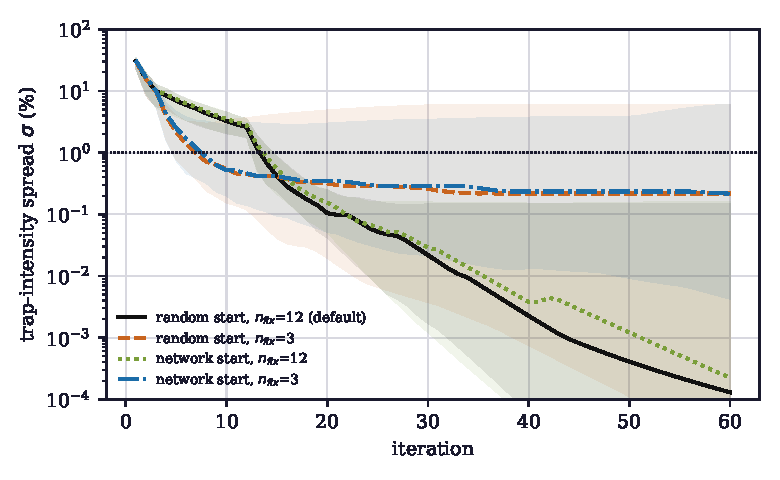
\includegraphics[width=0.78\textwidth]{fig-traces.pdf}
\caption{Median relative standard deviation of the trap intensities along the $\budget$ iterations of phase-fixed WGS on the $\nGeo$ held-out geometries, for the four arms (random or network start, $\nfix=3$ or $12$); the bands are the interquartile range across geometries and the dotted line is the 1\% threshold.}
\label{fig:traces}
\end{figure}

\begin{figure}[t]
\centering
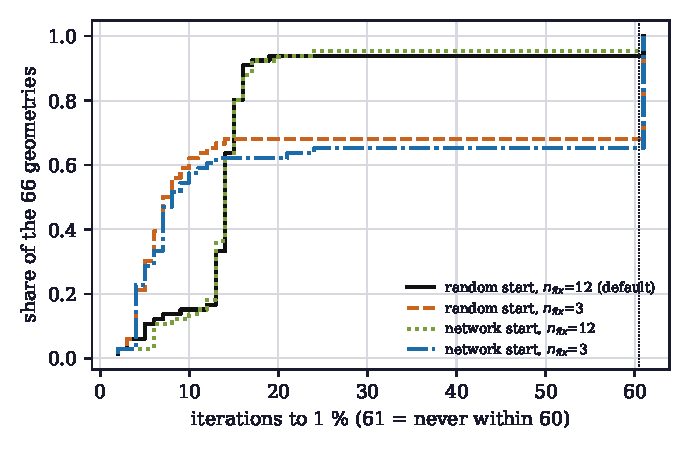
\includegraphics[width=0.62\textwidth]{fig-ecdf.pdf}
\caption{Empirical distribution of the iterations to 1\% over the $\nGeo$ held-out geometries for the four arms; the value $\budget+1$ marks the geometries that never reach 1\% within the budget, which is where the early-freeze arms leave about a third of the geometries.}
\label{fig:ecdf}
\end{figure}

\subsection{Geometry by geometry}\label{sec:res-paired}

Figure~\ref{fig:paired} compares the arms geometry by geometry. Against a random start with the same freeze index (Figure~\ref{fig:paired}a) the points lie on the diagonal: the network start needs the same number of iterations on \signTRThreeN{} of the $\nGeo$ geometries, fewer on \signARThreeN{} and more on \signBRThreeN{} (sign test $p=\signPRThreeN$), so if anything the network is slightly slower than the random start at $\nfix=3$, a difference that is not
distinguishable from none. Against the default (Figure~\ref{fig:paired}b) the network start needs fewer iterations on \signARN{} geometries and more on \signBRN{}, the latter being mostly geometries on which it does not converge at all. Of the \nGeo{} geometries, \capBoth{} reach the cap with both early-freeze arms, \capRNotN{} only with the random start and \capNNotR{} only with the network start. The medians separated by group are \genItRTwelve{} (random, $\nfix=12$), \genItRThree{} (random, $\nfix=3$) and \genItNThree{} (network, $\nfix=3$) on the generated geometries, and \benchItRTwelve{}, \benchItRThree{} and \benchItNThree{} on the six benchmark geometries.

\begin{figure}[t]
\centering
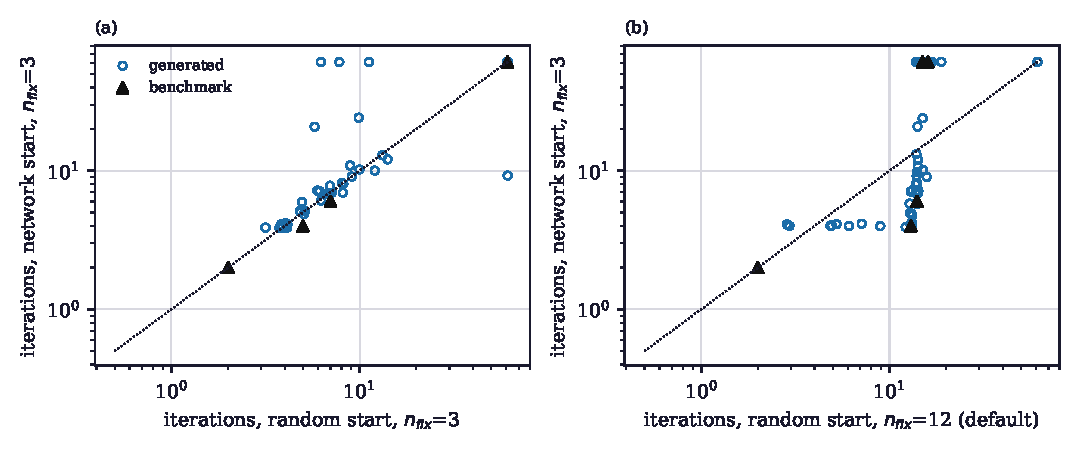
\includegraphics[width=\textwidth]{fig-paired.pdf}
\caption{Iterations to 1\% per held-out geometry, network start at $\nfix=3$ (vertical axis) against (a) the random start at $\nfix=3$ and (b) the random start at the default $\nfix=12$ (horizontal axis), logarithmic axes, with a small jitter for ties; circles are generated geometries, triangles the six benchmark geometries, the dotted line is equality and $\budget+1$ marks a run that never reaches 1\%.}
\label{fig:paired}
\end{figure}

\section{Ablation}\label{sec:ablation}

\subsection{Network start against early freeze}\label{sec:abl-four}

The candidate changed two things at once with respect to the published default: the start phases and the freeze index. Table~\ref{tab:ablation} separates them on the same $\nGeo$ geometries and seeds, and Figure~\ref{fig:ablation} shows the medians with their intervals and the share of runs that never reach 1 percent.
The early freeze alone, with no network, lowers the median from \itRTwelve{} to \itRThree{} iterations, a factor of \ratioRoverRThree{} (interval \ratioRoverRThreeLo{} to \ratioRoverRThreeHi), and the paired sign test over geometries rejects equality ($\signARRThree$ geometries need more iterations with the default, $\signBRRThree$ fewer, $\signTRRThree$ ties, $p=\signPRRThree$). The network alone, with the published freeze, does not change the median (\itNTwelve{} against \itRTwelve, factor \ratioRoverNTwelve{}; $\signARNTwelve$ against $\signBRNTwelve$ geometries, $p=\signPRNTwelve$). The combination of the two, the candidate, gives \itNThree{} iterations, a factor of
\ratioRoverN{}, which is below the factor of the early freeze alone (\ratioRoverRThree{}), and its sign test against the default has $p=\signPRN$, larger than that of the freeze alone. In every comparison the arm with the network is not better than the arm without it that has the same freeze index.

\begin{table}[t]
\centering\small
\resizebox{\textwidth}{!}{\begin{tabular}{@{}lccrrr@{}}
\toprule
Arm & Network start & Early freeze & Median it. & Ratio to the default [95\% CI] & Sign test $p$ \\
\midrule
engine default & no & no & 14 & 1 & -- \\
early freeze only & no & yes & 7.5 & 1.87 [1.38, 2.33] & 0.0032 \\
network only & yes & no & 14 & 1.00 [1.00, 1.00] & 0.29 \\
network and early freeze & yes & yes & 8 & 1.75 [0.85, 2.00] & 0.092 \\
\bottomrule
\end{tabular}
}
\caption{Ablation of the learned warm start on the $\nGeo$ held-out geometries: the network start and the early freeze index ($\nfix=3$ against the default 12) crossed, with the median iterations to 1\%, the ratio of the default's median to each arm's with a bootstrap 95\% interval, and the exact two-sided sign test against the default.}
\label{tab:ablation}
\end{table}

\begin{figure}[t]
\centering
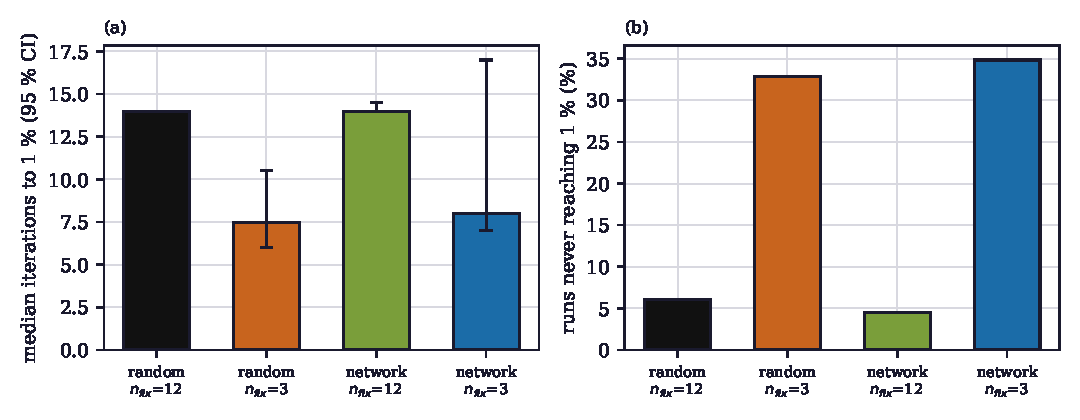
\includegraphics[width=\textwidth]{fig-ablation.pdf}
\caption{Ablation on the $\nGeo$ held-out geometries: (a) median iterations to 1\% with the bootstrap 95\% interval for the four arms; (b) share of the runs ($\nGeo$ geometries, $\nSeeds$ seeds) that do not reach 1\% within \budget{} iterations, which is the price of the early freeze whatever the start.}
\label{fig:ablation}
\end{figure}

The efficiency tells the same story. The final efficiency is \effmRTwelve{} at the default, \effmNTwelve{} for the network at $\nfix=12$ and \effmRThree{} and \effmNThree{} with the early freeze: the loss of efficiency that failed H2 is caused by the freeze (\effdRThree{} percent for a random start with it) and the network adds \effdNThreeRThree{} percent to it. The share of runs that never reach 1 percent shows what the early freeze buys the median with: \neverRThree{} percent for the random start at $\nfix=3$ and \neverNThree{} percent for the network, against \neverRTwelve{} and \neverNTwelve{} percent at the default.
A statistic that does not look at the tail, the median, hides that the early freeze fails to converge on about a third of the runs.

\subsection{Sweep of the freeze index}\label{sec:abl-sweep}

Table~\ref{tab:sweep} and Figure~\ref{fig:sweep} give the median iterations, the share that never converge and the final spread for the freeze index from $1$ to $12$, for both starts, on the $30$ geometries of the sweep. The median for the random start falls from \swTwelve{} iterations at $\nfix=12$ to \swEight{} at $8$, \swSix{} at $6$, \swFour{} at $4$ and \swThree{} at $3$, while the share of runs that never reach 1 percent rises from \swTwelveNever{} to \swEightNever{}, \swSixNever{}, \swFourNever{} and \swThreeNever{} percent. At $\nfix=2$ the median is the cap (the run does not converge on most geometries) and at $\nfix=1$ it is too:
\swOneNever{} percent of the runs never converge. The final spread rises as the freeze index falls, from \swTwelveFin{} percent at 12 to \swThreeFin{} at 3. The relation is a trade between iterations and the probability of reaching 1 percent, with a minimum of the median near $\nfix=4$.

The network start follows the random start along the whole sweep. At $\nfix=1$, where Proposition~\ref{prop:washout}(a) says the run is a function of the start phases alone and the network would have its fullest effect, the network start reaches 1 percent in the median in \swnOne{} iterations and fails to converge in \swnOneNever{} percent of the runs, against \swOneNever{} percent for the random start. At $\nfix=2$ the shares are \swnTwoNever{} and \swTwoNever{} percent, at $\nfix=3$ \swnThreeNever{} and \swThreeNever{}, at $\nfix=4$ \swnFourNever{} and \swFourNever{}, at $\nfix=6$ \swnSixNever{} and \swSixNever{} and at $\nfix=12$ \swnTwelveNever{} and \swTwelveNever{}. The medians differ by at most one iteration
wherever both are below the cap. The final spread of the network is lower than the random start's at several indices on this subset (at $\nfix=12$, \swnTwelveFin{} against \swTwelveFin{} percent), but it is higher over the full $\nGeo$ geometries (\finNTwelve{} against \finRTwelve{} percent), so the direction of the final-spread difference is not consistent and we do not claim one.

\begin{table}[t]
\centering\small
\resizebox{\textwidth}{!}{\begin{tabular}{@{}rrrrrrr@{}}
\toprule
$n_{\mathrm{fix}}$ & Random: median it. & Never (\%) & Final $\sigma$ (\%) & Network: median it. & Never (\%) & Final $\sigma$ (\%) \\
\midrule
1 & 61 & 76.7 & 34.3 & 61 & 80 & 52.2 \\
2 & 61 & 61.1 & 2.32 & 61 & 70 & 20.1 \\
3 & 9.5 & 41.1 & 0.512 & 10.5 & 40 & 0.213 \\
4 & 8 & 28.9 & 0.202 & 9 & 23.3 & 0.18 \\
6 & 10 & 14.4 & 0.0742 & 10 & 20 & 0.0371 \\
8 & 11 & 12.2 & 0.00997 & 12 & 16.7 & 0.0352 \\
12 & 14 & 7.8 & 0.00013 & 14 & 6.7 & 1.91e-05 \\
\bottomrule
\end{tabular}
}
\caption{Sweep of the freeze index $\nfix$ on 30 of the held-out geometries (every second generated geometry, $\nSeeds$ seeds): median iterations to 1\% (the value 61 means the median run does not reach 1\% within 60 iterations), share of runs that never reach it and median final spread, for a random start and for the network start.}
\label{tab:sweep}
\end{table}

\begin{figure}[t]
\centering
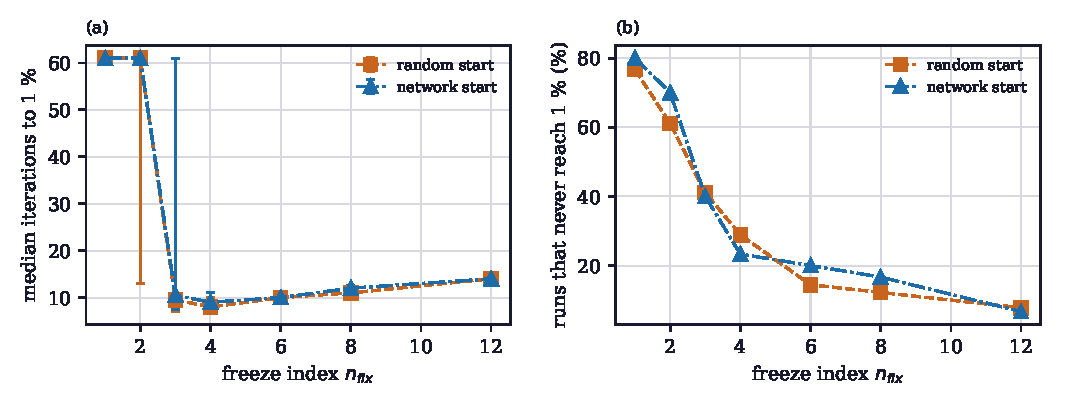
\includegraphics[width=\textwidth]{fig-sweep.pdf}
\caption{Sweep of the freeze index $\nfix$ on 30 held-out geometries for the random and the network start: (a) median iterations to 1\% with the bootstrap 95\% interval; (b) share of runs that never reach 1\% within \budget{} iterations. The two starts follow each other at every index.}
\label{fig:sweep}
\end{figure}

\subsection{Oracle start}\label{sec:abl-oracle}

The strongest start a predictor could be asked for is the converged solution of the iteration itself. Table~\ref{tab:oracle} and Figure~\ref{fig:oracle} give, for ten generated geometries and the first seed, the iterations to 1 percent from the phases of a converged random-start run. With the default freeze, the oracle start needs a median of \OTwelveMed{} iterations against \ORMed{} from the random start, a saving of \OTwelveGain{} iteration; at $\nfix=3$ it needs \OThreeMed{} against \ORThreeMed{}, and with the freeze at the first iteration \OOneMed{}. On the geometry that does not converge for
any arm (the largest array of the ten, \texttt{gen/06} in Table~\ref{tab:oracle}) the oracle does not help either. Two readings follow. First, at the published freeze index the start cannot be worth more than about one iteration, whoever predicts it: the network at $\nfix=12$ has nothing to improve. Second, with an oracle the early freeze converges on geometries on which the random start with the same freeze never does (\texttt{gen/01}, \texttt{gen/03} and \texttt{gen/08}), which is the part of the gap a perfect predictor could close; the network, with its phases, does not close it (Table~\ref{tab:sweep}). The predicted
phases are not those of a converged solution, which the trap list alone does not determine because the converged phases of a dense array depend on the random start that produced them.

\begin{table}[t]
\centering\small
\resizebox{\textwidth}{!}{\begin{tabular}{@{}lrrrrrr@{}}
\toprule
Held-out geometry & Traps & Random, 12 & Oracle, 12 & Random, 3 & Oracle, 3 & Oracle, 1 \\
\midrule
gen/00 & 236 & 13 & 11 & 7 & 5 & 5 \\
gen/01 & 345 & 18 & 14 & 61 & 8 & 8 \\
gen/02 & 448 & 14 & 13 & 16 & 6 & 6 \\
gen/03 & 456 & 15 & 13 & 61 & 7 & 6 \\
gen/04 & 133 & 14 & 13 & 7 & 5 & 5 \\
gen/05 & 102 & 13 & 13 & 5 & 5 & 4 \\
gen/06 & 768 & 61 & 61 & 61 & 61 & 61 \\
gen/07 & 679 & 13 & 8 & 4 & 4 & 4 \\
gen/08 & 450 & 16 & 14 & 61 & 9 & 8 \\
gen/09 & 140 & 5 & 2 & 4 & 2 & 2 \\
\bottomrule
\end{tabular}
}
\caption{Iterations to 1\% on ten held-out geometries (first seed) from a random start and from the oracle start (the phases of a converged random-start run) for freeze indices 12, 3 and 1; the value 61 means 1\% is not reached within 60 iterations.}
\label{tab:oracle}
\end{table}

\begin{figure}[t]
\centering
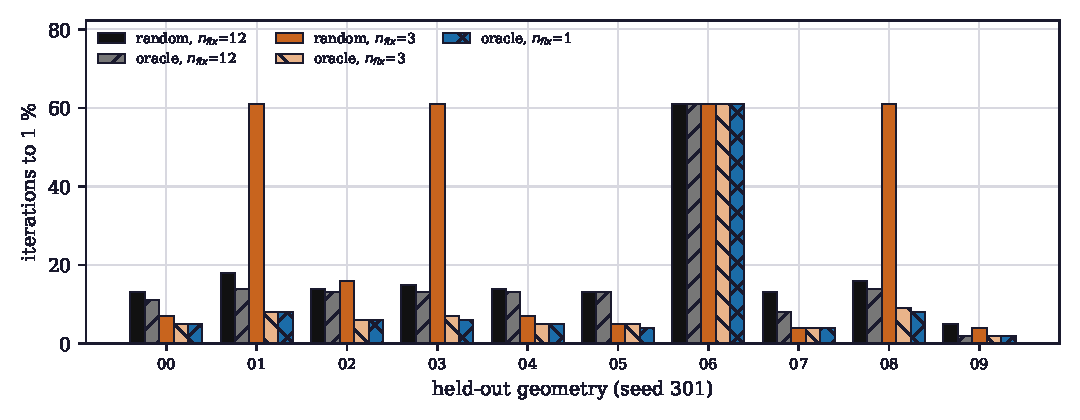
\includegraphics[width=\textwidth]{fig-oracle.pdf}
\caption{Iterations to 1\% on ten held-out geometries from a random start and from the oracle start for freeze indices 12, 3 and 1 (first seed); the bars at the top of the axis are runs that do not reach 1\% within the budget.}
\label{fig:oracle}
\end{figure}

\subsection{Weight accounting}\label{sec:abl-weights}

Table~\ref{tab:weights} and Figure~\ref{fig:weights} apply Proposition~\ref{prop:allowance} to the runs of the oracle comparison. The bound of Eq.~\eqref{eq:allowance} holds on all \wTwelveHold{} of \wTwelveN{} runs of each of the four conditions. It is loose: the weight spread of a converged run, a median of \wTwelveSMed{} for the random start at $\nfix=12$, is within reach of the allowance after a median of \wTwelveKMed{} iterations ($k_{\mathrm{floor}}$), while the median run needs \wTwelveItMed{} iterations to reach 1 percent. With an oracle start at $\nfix=12$ the corresponding numbers are \woTwelveKMed{} and
\woTwelveItMed{}. The restart of the weights at one therefore does not explain why 1 percent arrives at iteration 13 or later: the accounting identity permits the weights to rebuild their spread long before. This rules out the explanation that the weights, which restart, are the bottleneck, and it points to the freeze index as the quantity that sets the iteration count.

\begin{table}[t]
\centering\small
\resizebox{\textwidth}{!}{\begin{tabular}{@{}lrrrr@{}}
\toprule
Run (seed 301, ten geometries) & Median final $S$ & Median $k_{\mathrm{floor}}$ & Median it. to 1\% & Bound holds \\
\midrule
random start, $n_{\mathrm{fix}}=12$ & 0.71 & 2 & 14 & 10 of 10 \\
random start, $n_{\mathrm{fix}}=3$ & 1.43 & 3 & 11.5 & 10 of 10 \\
oracle start, $n_{\mathrm{fix}}=12$ & 0.67 & 4 & 13 & 10 of 10 \\
oracle start, $n_{\mathrm{fix}}=3$ & 0.80 & 5.5 & 5.5 & 10 of 10 \\
\bottomrule
\end{tabular}
}
\caption{Weight accounting on ten held-out geometries (first seed): median final log-spread $S$ of the weights, the first iteration $k_{\mathrm{floor}}$ at which the cumulative allowance of Eq.~\eqref{eq:allowance} reaches that spread, the median iterations to 1\%, and the number of runs on which the bound holds, for the random and the oracle start at two freeze indices.}
\label{tab:weights}
\end{table}

\begin{figure}[t]
\centering
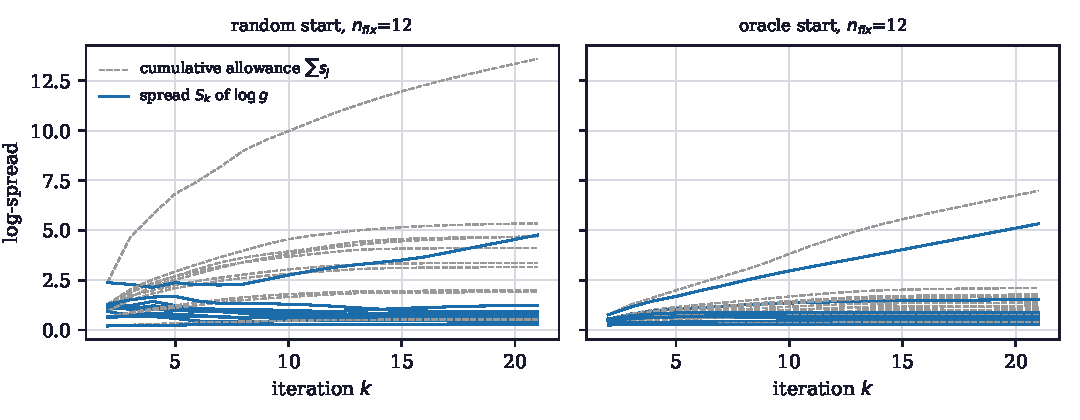
\includegraphics[width=\textwidth]{fig-weights.pdf}
\caption{Log-spread $S_k$ of the weights after iteration $k$ (solid) and the cumulative allowance $\sum_{j\le k}s_j$ of Eq.~\eqref{eq:allowance} (dashed), for ten held-out geometries at $\nfix=12$, from the random start (left) and the oracle start (right); the solid curves stay below the dashed ones on every run.}
\label{fig:weights}
\end{figure}

\section{Discussion}\label{sec:discussion}

\subsection{Why the network does not help}\label{sec:why-not}

The measurements give three reasons, in decreasing order of how directly they are measured. First, the iteration the network feeds forgets its start. At the published freeze index the run of the iteration passes through eleven applications of the update before the focal phase is frozen (Proposition~\ref{prop:washout}), and the phases of a converged run, the best start that was constructed, save \OTwelveGain{} iteration on ten geometries and one seed (Table~\ref{tab:oracle}), which is consistent with a small value of a phase predictor at $\nfix=12$ and is not a bound over all starts, and the network at $\nfix=12$ saves none (Table~\ref{tab:ablation}).
Second, where the start does matter, at an early freeze, what matters is whether the frozen phases are compatible with a uniform solution, and whether the trap list determines such phases is not tested here: the oracle start, whose converged phases the trap list does not supply, converges on geometries where a random start does not and halves the median at $\nfix=3$ (\ORThreeMed{} to \OThreeMed{}), while the network, trained on a loss that rewards low spread after ten iterations, does not (Table~\ref{tab:sweep}, Table~\ref{tab:oracle}). That headroom of a factor of two is the open question that this network leaves. Third, the training objective did not transfer to the held-out geometries: during training the network lowered the spread after the first iteration
from \trainSigRandFirst{} to \trainSigNetFirst{} percent on the training distribution, an advantage that is gone by iteration ten (\trainSigNet{} against \trainSigRand{} percent) and absent after the first iteration on the held-out geometries (\trNThreeOne{} against \trRTwelveOne{} percent). We cannot say from these runs whether a longer or differently designed training would move the third reason; the first two do not depend on the training.

\subsection{The gain belongs to the freeze index}\label{sec:freeze-gain}

The reduction in median iterations that the candidate shows with respect to the default is real and is reproduced without a network: a random start with the same early freeze needs \itRThree{} iterations. The sweep of Section~\ref{sec:abl-sweep} puts it in context: the median iterations fall steadily as the freeze index falls from 12 to 4 and the share of runs that never converge rises at the same time, from \swTwelveNever{} to \swFourNever{} percent. An early freeze is a bet that the phases at that moment are good
enough, and on this model the bet fails on a share of the geometries that grows as the freeze comes earlier. A practitioner who wants fewer iterations on arrays of the type of the held-out set can therefore lower $\nfix$ and accept the failure share; we did not test any remedy for the failed runs, such as a restart with a later freeze, and we make no recommendation. The default of Kim et al.~\cite{kim2019} was chosen on their own array and camera; we did not test their array, and nothing in these results says that their choice was suboptimal for it. What the results say
is that on the dense generated arrays of this study, in the scalar model, the default is a conservative point of a trade between iterations and reliability, and a learned start does not move the trade.

\subsection{Cost of the network against what it can save}\label{sec:cost}

By operation count (Section~\ref{sec:complexity}) the network pass costs of the order of two iterations of the point form at the largest array of 1024 traps and less on smaller ones, because its attention is quadratic in $M$ while an iteration is linear in it. A start that saved about one iteration at $\nfix=12$ would not repay a pass of that size on the largest arrays, and for arrays of a hundred traps the pass is much cheaper than an iteration, so the net balance is a question of the array size and of the saving, which is zero here. We did not measure the inference time of the exported graph in a browser, so the cost statement is an operation count, not a timing.

The balance is different for the many holograms of a sequence, where each hologram starts from its predecessor and no start has to be predicted, and for arrays smaller than a hundred traps, where the iteration is cheap and the median iterations to 1 percent are already few. The cost statement therefore holds for the dense, large arrays for which a warm start was proposed, which are also the arrays where the pass is the most expensive.

\subsection{The explanation by the weights}\label{sec:error}

The hypothesis that a warm start should be hard because the weights restart at one is not supported by the accounting of Section~\ref{sec:abl-weights}: the allowance permits the weights to rebuild their spread in \wTwelveKMed{} iterations, far before 1 percent arrives. The iteration count is set by the freeze, not by the rebuilding of the weights, in the data of this study. The hypothesis follows from the structure of the iteration and was tested by the measurement of Table~\ref{tab:weights}, which did not support it. The proposition is a true inequality and stays; the hypothesis is dropped. An explanation that follows from the structure of an algorithm is a hypothesis, and the quantity it predicts (here a lower bound on the iterations) can be computed on every run at no cost; computing it shows that the bound is far below the observed counts. The same accounting applied to the oracle start gives the same answer, so the conclusion does not depend on the quality of the start. What the accounting leaves open is why the freeze index sets the count, for which the evidence is that of Conjecture~\ref{conj:freeze}, with its counterexamples, and no proof.

\subsection{What the result does not close}\label{sec:open}

A label-based warm start (regressing converged phases on a family of geometries where they are determined, for instance regular lattices) or a modified freeze rule that lets a start carry information through the iteration would be different designs, not tunings of this one, and the results here neither support nor exclude them. What the data suggest as a quantity to look for in a future design is the largest freeze index at which a given start still converges, and the share of geometries on which it does not. A start that moved that curve, one that converged on the geometries where a random start with an early freeze fails, would be a warm start in the sense of the proposal; the oracle start does it on three geometries of ten, and the network start does it on \capRNotN{} of the \nGeo{} held-out geometries while failing on \capNNotR{} where the random start with the same freeze converges. We also did not test whether a network trained at the published freeze index with a longer unroll would behave differently from the candidate; the single earlier trial at that setting reached about the random level, and it is the only evidence we have on the question. The oracle start suggests a saving of about one iteration for phase starts at the published freeze on these ten geometries, but it is one particular start (the converged phases of a single random-start run, one seed), so it is not a bound over all starts.

\section{Limitations and threats to validity}\label{sec:limits}

\subsection{Internal validity}\label{sec:internal}

The negative result concerns one trained network: one architecture (a two-block set transformer of width 64), one training run of $\trainSteps$ steps with one initialization seed and one data seed, one loss (Eq.~\eqref{eq:loss}) and one training freeze index ($\nfix=3$). We did not train other widths, depths, losses, unroll lengths or freeze indices for this study, so we cannot say that no network of the family would do better; a negative result on one candidate is a negative result on that candidate.
The variation across the training seeds, which would give the uncertainty of the network's contribution itself, was not measured. The evaluation has $\nGeo$ geometries and $\nSeeds$ seeds, and the integer-valued, capped statistic produces coarse medians: the intervals of the arms with the early freeze are wide (\itNThreeLo{} to \itNThreeHi{} for the candidate) because the distribution of $k_1$ is bimodal, with a mass near the median and a mass at the cap. The sign test is the more informative comparison here, and we report both.

The ablation was designed after the first evaluation had failed (hypothesis H4), so its tests are exploratory; the sweep and the oracle start were added for the same reason. The sweep and the weight accounting use subsets (30 and ten geometries) that were chosen by position in the generated list, not at random, and the oracle start uses one seed. The numbers of the sweep, the oracle and the accounting carry no intervals beyond those shown.

\subsection{External validity}\label{sec:external}

The model is the scalar Fourier model with ideal pixels (Section~\ref{sec:assumptions}), without pixel crosstalk, phase quantization, flicker or an input beam other than the Gaussian one; an instrument adds effects that change the trap intensities after the hologram is computed and that camera feedback absorbs, and the number of iterations of the phase-fixed iteration on a real device is not what we measure. The geometries are point traps without vortices, at most 1024 in number, on grids of $256^2$ and $512^2$ pixels; the held-out set is filtered to be demanding for the random start of the default iteration, so the conclusion holds for dense arrays that need more than three iterations and says nothing about sparse arrays, which any start solves in one.
The training generators and the held-out generated geometries are the same families with different seeds, so the held-out set tests generalization over instances of the families and over the unseen benchmark families only in as far as the six benchmark geometries show; six geometries do not give a statistic.

\subsection{Construct validity}\label{sec:construct}

The cost of a hologram is measured as iterations to 1 percent of the relative standard deviation, with a cap. Iterations are the unit of the acceptance test, but they are not time: the network pass has a cost (Section~\ref{sec:cost}) that was counted but not timed, and iterations do not show that the early freeze lowers the final efficiency by about \effdRThree{} percent. A threshold other than 1 percent would give other counts; we did not sweep it. The median over geometries of the median over seeds is the statistic of the acceptance test; we kept it for comparability and added the share of runs that do not reach the threshold, which the median hides.

A final construct concern is the choice of the baseline: the random start of the published default, run by the engine of the product with the portable generator, is the reference of the acceptance test. Another implementation of the same iteration, with a different random generator, would give different seeds but the same distribution of runs; the engine implementation of the iteration was compared with an independent implementation by the product, and we did not rerun that comparison here.

\subsection{Scope of the claim}\label{sec:scope}

The claim that the study sustains is the following. On the held-out geometries of this study, in the scalar Fourier model, a network start trained as described does not reduce the iterations of phase-fixed WGS to 1 percent by the factor of two that the acceptance test required, and its gain at an early freeze is the gain of the early freeze without a network. The claim does not extend to other networks, other devices, hardware, other thresholds or a different iteration. It does not say that learned initializations cannot help other iterative hologram methods, which we did not test. The statement is tied to the held-out set, to the three seeds and to the budget of $\budget$ iterations, and every number that sustains it is produced by the script of Section~\ref{sec:repro}. The model is not released, and the product's slot for it answers with the random start of the iteration.

\section{Reproducibility}\label{sec:repro}
\sloppy

The code, the committed records and the scripts that regenerate every number, table and figure of this paper are in the repository \url{https://github.com/fsantibanezleal/CEFOP_DinHot} (Apache-2.0), under \texttt{manuscripts/learned-warm-start/}. The studio that hosts the method runs at \url{https://dinhot.fasl-work.com}. The record of the rejected candidate is \texttt{data/derived/models/warmstart-model-rejected.json}; the method is the module \texttt{b3\_warm\_start.py}, and the held-out set, the training and the evaluation are in the package \texttt{learned/} of the engine.

\textbf{Commands.} From the repository root, with the GPU environment of the product (it holds PyTorch; only the CPU is used by the measurement):
\begin{itemize}
\item \texttt{python manuscripts/learned-warm-start/data/measure.py --workers 12} runs every arm, the sweep, the oracle start and the weight accounting, and writes \texttt{warm.json}, \texttt{warm\_numbers.tex} and the table files; it took \runtimeMin{} minutes with \nWorkers{} worker processes on the workstation of Section~\ref{sec:hardware}. With \texttt{--emit-only} it rewrites the macro and table files from \texttt{warm.json} without rerunning.
\item \texttt{python manuscripts/learned-warm-start/figures/make\_figs.py} regenerates the nine vector figures from \texttt{warm.json}.
\item Three passes of \texttt{pdflatex} in \texttt{manuscripts/learned-warm-start/tex/} build the paper.
\end{itemize}

\textbf{Data and artifacts.} The held-out file and the checkpoint of the candidate are in the learned directory of the data root, named by the environment variable \texttt{DINHOT\_LEARNED\_DIR}; they are not in the repository. The held-out file is regenerated bit for bit by the function \texttt{build\_warm} of \texttt{learned/heldout.py} from its recorded seeds, and its sha256 digest, which the measurement script checks against the committed record before it runs, is the identity check. The checkpoint comes from the training function of Algorithm~\ref{alg:train} with the data seed 20261101 and the initialization seed 7; the exported graph is not committed because the model is not released. Every random choice goes through the portable seeded generator of the engine, so a rerun reproduces the numbers up to the floating point of the machine's fast Fourier transform. The numbers of the text are macros written by the measurement script, so none of them is typed.

\section{Conclusions}\label{sec:conclusions}

We built a learned warm start for phase-fixed weighted Gerchberg--Saxton: a permutation-equivariant set network with \nParams{} parameters that predicts one initial phase per trap, trained without labels through an unrolled copy of the iteration, with an acceptance test fixed in advance. On $\nGeo$ held-out geometries it does not meet the test. The network start with an early phase freeze reaches a relative standard deviation of 1 percent in a median of \itNThree{} iterations (95\% interval \itNThreeLo{} to \itNThreeHi) against \itRTwelve{} for the random start of the published method, a factor of \ratioRoverN{} (interval \ratioRoverNLo{} to \ratioRoverNHi) where two was required,
and its final efficiency is \effdNThree{} percent from the published method's where 1 percent was allowed.

The four-arm ablation attributes the gain to the freeze index and not to the network: a random start with the same early freeze needs \itRThree{} iterations, the network at the published freeze index needs \itNTwelve{}, and a start from the phases of a converged run saves only \OTwelveGain{} iteration at that index. The early freeze has a price that the median hides: \neverRThree{} percent of the runs never reach 1 percent within \budget{} iterations, against \neverRTwelve{} percent for the published default, and the final efficiency is about \effdRThree{} percent lower. The accounting bound on the weights holds on every run and is loose, so the restart of the weights does not explain the iteration count; the freeze index does.

The model is not released. The questions that remain are different designs, not tunings: a start trained on labels where converged phases are determined, or a change of the freeze rule that lets a start carry information through the iteration. The results hold on a scalar Fourier model of the device and for one trained network; the experiment that would extend them is a measurement on an instrument with its device model and camera feedback, and a study of the variation across training seeds.

\begin{thebibliography}{99}\small
\bibitem{gs1972} R.~W.~Gerchberg and W.~O.~Saxton, ``A practical algorithm for the determination of phase from image and diffraction plane pictures,'' \emph{Optik} 35(2), 237--246, 1972 (no DOI; scan: \url{https://web.archive.org/web/20160328053000/http://www.u.arizona.edu/~ppoon/GerchbergandSaxton1972.pdf}).
\bibitem{dileonardo} R. Di Leonardo, F. Ianni and G. Ruocco, ``Computer generation of optimal holograms for optical trap arrays,'' \emph{Opt. Express} 15(4), 1913, 2007. \url{https://doi.org/10.1364/OE.15.001913}.
\bibitem{bianchi} S. Bianchi and R. Di Leonardo, ``Real-time optical micro-manipulation using optimized holograms generated on the GPU,'' \emph{Comput. Phys. Commun.} 181(8), 1444--1448, 2010. \url{https://doi.org/10.1016/j.cpc.2010.04.012}.
\bibitem{polin} M. Polin, K. Ladavac, S.-H. Lee, Y. Roichman and D. G. Grier, ``Optimized holographic optical traps,'' \emph{Opt. Express} 13(15), 5831, 2005. \url{https://doi.org/10.1364/OPEX.13.005831}.
\bibitem{whyte} G. Whyte and J. Courtial, ``Experimental demonstration of holographic three-dimensional light shaping using a Gerchberg--Saxton algorithm,'' \emph{New J. Phys.} 7, 117, 2005. \url{https://doi.org/10.1088/1367-2630/7/1/117}.
\bibitem{kim2019} D.~Kim \emph{et al.}, ``Large-scale uniform optical focus array generation with a phase spatial light modulator,'' \emph{Opt. Lett.} 44(12), 3178, 2019. \url{https://doi.org/10.1364/OL.44.003178}.
\bibitem{kimoe} H.~Kim, M.~Kim, W.~Lee and J.~Ahn, ``Gerchberg--Saxton algorithm for fast and efficient atom rearrangement in optical tweezer traps,'' \emph{Opt. Express} 27(3), 2184, 2019. \url{https://doi.org/10.1364/OE.27.002184}.
\bibitem{lee} W.~Lee, H.~Kim and J.~Ahn, ``Defect-free atomic array formation using the Hungarian matching algorithm,'' \emph{Phys. Rev. A} 95(5), 053424, 2017. \url{https://doi.org/10.1103/PhysRevA.95.053424}.
\bibitem{lpi} I.~H.~A.~Knottnerus, Y.~C.~Tseng, A.~Urech, R.~J.~C.~Spreeuw and F.~Schreck, ``Parallel assembly of neutral atom arrays with an SLM using linear phase interpolation,'' \emph{SciPost Phys.} 19(4), 118, 2025. \url{https://doi.org/10.21468/SciPostPhys.19.4.118}.
\bibitem{nogrette} F.~Nogrette \emph{et al.}, ``Single-atom trapping in holographic 2D arrays of microtraps with arbitrary geometries,'' \emph{Phys. Rev. X} 4(2), 021034, 2014. \url{https://doi.org/10.1103/PhysRevX.4.021034}.
\bibitem{chew} Y.~T.~Chew \emph{et al.}, ``Ultraprecise holographic optical tweezer array,'' \emph{Phys. Rev. A} 110(5), 053518, 2024. \url{https://doi.org/10.1103/PhysRevA.110.053518}.
\bibitem{ebadi} S.~Ebadi \emph{et al.}, ``Quantum phases of matter on a 256-atom programmable quantum simulator,'' \emph{Nature} 595, 227--232, 2021. \url{https://doi.org/10.1038/s41586-021-03582-4}.
\bibitem{manetsch} H.~J.~Manetsch, G.~Nomura, E.~Bataille, X.~Lv, K.~H.~Leung and M.~Endres, ``A tweezer array with 6,100 highly coherent atomic qubits,'' \emph{Nature} 647, 60--67, 2025. \url{https://doi.org/10.1038/s41586-025-09641-4}.
\bibitem{harte} T. Harte, G. D. Bruce, J. Keeling and D. Cassettari, ``Conjugate gradient minimisation approach to generating holographic traps for ultracold atoms,'' \emph{Opt. Express} 22(22), 26548, 2014. \url{https://doi.org/10.1364/OE.22.026548}.
\bibitem{bowman} D.~Bowman \emph{et al.}, ``High-fidelity phase and amplitude control of phase-only computer generated holograms using conjugate gradient minimisation,'' \emph{Opt. Express} 25(10), 11692, 2017. \url{https://doi.org/10.1364/OE.25.011692}.
\bibitem{wirtinger} P.~Chakravarthula, Y.~Peng, J.~Kollin, H.~Fuchs and F.~Heide, ``Wirtinger holography for near-eye displays,'' \emph{ACM Trans. Graph.} 38(6), 1--13, 2019. \url{https://doi.org/10.1145/3355089.3356539}.
\bibitem{schroff} P. Schroff, A. La Rooij, E. Haller and S. Kuhr, ``Accurate holographic light potentials using pixel crosstalk modelling,'' \emph{Sci. Rep.} 13, 3252, 2023. \url{https://doi.org/10.1038/s41598-023-30296-6}.
\bibitem{pasienski} M. Pasienski and B. DeMarco, ``A high-accuracy algorithm for designing arbitrary holographic atom traps,'' \emph{Opt. Express} 16(3), 2176, 2008. \url{https://doi.org/10.1364/OE.16.002176}.
\bibitem{holland} N.~Holland, D.~Stuart, O.~Barter and A.~Kuhn, ``Benchmarking modern algorithms to holographically create optical tweezers for laser-cooled atoms,'' \emph{J. Mod. Opt.} 65(18), 2133--2141, 2018 (preprint title ``Efficient and fast algorithms to generate holograms for optical tweezers,'' arXiv:1711.07845). \url{https://doi.org/10.1080/09500340.2018.1499978}.
\bibitem{swan} H.~Swan, A.~Torchylo, M.~J.~Van de Graaff, J.~Rudolph and J.~M.~Hogan, ``High-fidelity holographic beam shaping with optimal transport and phase diversity,'' \emph{Opt. Express} 33(3), 6290--6303, 2025. \url{https://doi.org/10.1364/OE.540901}.
\bibitem{torchylo} A.~Torchylo, H.~Swan, L.~Tellez and J.~M.~Hogan, ``A fast, large-scale optimal transport algorithm for holographic beam shaping,'' \emph{Opt. Express} 34(4), 6796--6803, 2026. \url{https://doi.org/10.1364/OE.588337}.
\bibitem{eybposh} M. H. Eybposh, N. W. Caira, M. Atisa, P. Chakravarthula and N. C. P\'egard, ``DeepCGH: 3D computer-generated holography using deep learning,'' \emph{Opt. Express} 28(18), 26636, 2020. \url{https://doi.org/10.1364/OE.399624}.
\bibitem{shi} L. Shi, B. Li, C. Kim, P. Kellnhofer and W. Matusik, ``Towards real-time photorealistic 3D holography with deep neural networks,'' \emph{Nature} 591, 234--239, 2021. \url{https://doi.org/10.1038/s41586-020-03152-0}.
\bibitem{peng} Y.~Peng, S.~Choi, N.~Padmanaban and G.~Wetzstein, ``Neural holography with camera-in-the-loop training,'' \emph{ACM Trans. Graph.} 39(6), 1--14, 2020. \url{https://doi.org/10.1145/3414685.3417802}.
\bibitem{ren} Z.~Ren \emph{et al.}, ``Creation of a tweezer array for cold atoms utilizing a generative neural network,'' \emph{APL Quantum} 1(4), 046111, 2024. \url{https://doi.org/10.1063/5.0219170}.
\bibitem{sambharya} R.~Sambharya, G.~Hall, B.~Amos and B.~Stellato, ``Learning to warm-start fixed-point optimization algorithms,'' arXiv:2309.07835, 2023 (preprint). \url{https://arxiv.org/abs/2309.07835}.
\bibitem{settransformer} J.~Lee, Y.~Lee, J.~Kim, A.~R.~Kosiorek, S.~Choi and Y.~W.~Teh, ``Set Transformer: a framework for attention-based permutation-invariant neural networks,'' International Conference on Machine Learning (ICML), 2019; arXiv:1810.00825. \url{https://arxiv.org/abs/1810.00825}.
\bibitem{deepsets} M.~Zaheer, S.~Kottur, S.~Ravanbakhsh, B.~Poczos, R.~Salakhutdinov and A.~Smola, ``Deep Sets,'' Neural Information Processing Systems (NIPS), 2017; arXiv:1703.06114. \url{https://arxiv.org/abs/1703.06114}.
\bibitem{fourierfeatures} M.~Tancik \emph{et al.}, ``Fourier features let networks learn high frequency functions in low dimensional domains,'' arXiv:2006.10739, 2020 (preprint). \url{https://arxiv.org/abs/2006.10739}.
\bibitem{adamw} I.~Loshchilov and F.~Hutter, ``Decoupled weight decay regularization,'' International Conference on Learning Representations (ICLR), 2019; arXiv:1711.05101. \url{https://arxiv.org/abs/1711.05101}.
\bibitem{efron} B. Efron, ``Bootstrap methods: another look at the jackknife,'' \emph{Ann. Statist.} 7(1), 1--26, 1979. \url{https://doi.org/10.1214/aos/1176344552}.
\bibitem{grimm} R.~Grimm, M.~Weidem\"uller and Y.~B.~Ovchinnikov, ``Optical dipole traps for neutral atoms,'' \emph{Adv. At. Mol. Opt. Phys.} 42, 95--170, 2000. \url{https://doi.org/10.1016/S1049-250X(08)60186-X}.
\end{thebibliography}


\end{document}
